\documentclass[12pt,letterpaper]{article}
\usepackage[T1]{fontenc}
\usepackage{mathptmx}  % newtx not installed in the build environment; mathptmx is the style-guide fallback
\renewcommand{\ttdefault}{lmtt}
\usepackage[letterpaper,margin=1in]{geometry}
\usepackage{amsmath,amssymb,amsthm}
\usepackage{microtype}
\usepackage{booktabs}
\usepackage{array}
\usepackage{enumitem}
\usepackage{tikz}
\usepackage[hidelinks]{hyperref}

\numberwithin{equation}{section}
\newtheorem{theorem}{Theorem}[section]
\newtheorem{proposition}[theorem]{Proposition}
\newtheorem{lemma}[theorem]{Lemma}
\newtheorem{corollary}[theorem]{Corollary}
\newtheorem{conjecture}[theorem]{Conjecture}
\theoremstyle{definition}
\newtheorem{definition}[theorem]{Definition}
\newtheorem{example}[theorem]{Example}
\newtheorem{algorithm}[theorem]{Algorithm}
\newtheorem{question}[theorem]{Question}
\theoremstyle{remark}
\newtheorem{remark}[theorem]{Remark}

% Remarks 2026.n: statements not fully verified in this revision
\newcounter{remxxvi}
\renewcommand{\theremxxvi}{2026.\arabic{remxxvi}}
\newenvironment{remarkxxvi}{\refstepcounter{remxxvi}\par\medskip\noindent
  \textbf{Remark~\theremxxvi.}\ }{\par\medskip}

\DeclareMathOperator{\wt}{wt}
\DeclareMathOperator{\supp}{supp}
\DeclareMathOperator{\ev}{ev}
\DeclareMathOperator{\codim}{codim}
\DeclareMathOperator{\vol}{vol}
\DeclareMathOperator{\conv}{conv}
\DeclareMathOperator{\GL}{GL}
\DeclareMathOperator{\Hom}{Hom}
\DeclareMathOperator{\divisor}{div}
\DeclareMathOperator{\Span}{span}
\newcommand{\F}{\mathbb{F}}
\newcommand{\Z}{\mathbb{Z}}
\newcommand{\Q}{\mathbb{Q}}
\newcommand{\R}{\mathbb{R}}
\newcommand{\PP}{\mathbb{P}}
\newcommand{\Fq}{\mathbb{F}_q}
\newcommand{\Fqs}{\mathbb{F}_q^{\times}}
\newcommand{\RM}{\mathcal{R}}
\newcommand{\OO}{\mathcal{O}}
\newcommand{\Lq}{\Lambda_q}
\newcommand{\st}[1]{\textup{(\emph{#1})}}

\title{Toric codes over finite fields\\[4pt]
\large Draft 5. Corrected and expanded version}
\author{David Joyner\thanks{\texttt{wdjoyner@gmail.com}.
The original version of this paper appeared as D.~Joyner, ``Toric codes over
finite fields,'' \emph{Applicable Algebra in Engineering, Communication and
Computing} \textbf{15} (2004), 63--79, preprint arXiv:math/0208155. It was
revised from the manuscript \texttt{toric\_code7.tex} dated September 1, 2003.
This corrected and expanded version was prepared in November 2026.}}
\date{November 22, 2026\\
Original draft: 2004. Corrected and expanded draft: 2026.}

\begin{document}
\maketitle

\begin{abstract}
This corrected and expanded version was prepared with substantial help from AI
systems (Anthropic's Claude as reviser, OpenAI's ChatGPT as referee). The
Acknowledgments give details. We associate error-correcting codes to toric
surfaces over a finite field $\Fq$, in analogy with the Goppa codes of a
curve. Evaluated on the full torus $T(\Fq)\cong(\Fqs)^2$, such a code depends
only on the residues modulo $q-1$ of the lattice points of a polygon. We show
that its dimension is the number of these residues and that its dual is again
a code of the same kind. We give short self-contained proofs of the
minimum distances of three of J.~Hansen's families. The proofs use a
grid-counting lemma of Alon--F\"uredi type, which also gives upper and lower
bounds on the minimum distance. We show by examples that two natural lower
bounds in terms of the volume or the number of lattice points of the polygon
do not hold. We give an error-locator decoding algorithm, in the form of an
error-correcting-pair algorithm with explicit toric hypotheses. We compute the
parameters of many examples exactly. In particular the $[49,11,28]$ code over
$\F_8$, which was better than all codes in the tables of 2002, has minimum
distance $28$ by exhaustive computer enumeration, for which we supply
independent verification scripts. The decoding algorithm corrects up to $5$
errors in this code in a fully worked example, and up to $6$ errors with a
pair found by computer search. A final section discusses connections with
graph theory.
\end{abstract}

\tableofcontents

%======================================================================
\section{Introduction}\label{sec:intro}

This section recalls the basic coding-theoretic vocabulary, gives the
Reed--Muller codes as a guiding example, and summarizes the results of the
paper.

Some of the constructions discussed here were implemented in
MAGMA~\cite{BCP97} and in GAP~\cite{GAP00} with the \textbf{toric}
package~\cite{Jo02}. GUAVA version 1.7 and later contain the toric-code
commands needed for the constructions~\cite{GUA02}. Every number in the
present version was recomputed independently with the scripts described in
Section~\ref{sec:summary}.

Let $\F=\Fq$ denote the finite field with $q$ elements. A \emph{$q$-ary code}
is, for us, a short exact sequence of vector spaces
\begin{equation}\label{eqn:1}
0 \longrightarrow C \xrightarrow{\ \gamma\ } \F^n
\xrightarrow{\ \theta\ } \F^{n-k} \longrightarrow 0 .
\end{equation}
We identify $C$ with its image under $\gamma$. If $\F^n$ has its standard
basis, then the matrix of $\gamma$ is a generator matrix of $C$ and the matrix
of $\theta$ is a parity check matrix of $C$. The integer $n$ is the
\emph{length} of $C$ and $k=\dim_{\F}C$ is its \emph{dimension}. A
\emph{codeword} is an element of $C$. Since \eqref{eqn:1} is exact, a vector
$v\in\F^n$ is a codeword if and only if $\theta(v)=0$. The \emph{Hamming
distance} between two vectors is the number of coordinates where they differ.
The \emph{weight} $\wt(v)$ of $v$ is its distance from $0$. The smallest
nonzero weight of a codeword is the \emph{minimum distance} $d=d(C)$. We call
$C$ an $[n,k,d]_q$ code.

In this paper we use toric varieties to construct codes. For one particular
choice of $n$, $k$ and $q$ the construction gave, in 2002, a value of $d$
larger than any previously known (Example~\ref{example:fan7}). We begin with a
related classical family.

\begin{example}[Generalized Reed--Muller codes]\label{example:RM}
Let $m\ge1$ and $0\le\ell\le m(q-1)$. Let $R=\F[x_1,\dots,x_m]_{\ell}$ be the
space of polynomials of total degree at most $\ell$ in which every variable
occurs with exponent at most $q-1$. Index the points of $\F^m$ as
$p_1,\dots,p_n$, so that $n=q^m$. The code
\[
\RM(\ell,m,q)=\{(f(p_1),\dots,f(p_n)) : f\in R\}
\]
is the \emph{generalized Reed--Muller code}. It was studied in this polynomial
form by Delsarte, Goethals and MacWilliams~\cite{DGM70}. Its dimension is the
number of monomials in $R$,
\[
k=\sum_{i=0}^{\ell}\ \sum_{j=0}^{\lfloor i/q\rfloor}(-1)^j\binom{m}{j}
\binom{m-1+i-qj}{m-1}.
\]
The inner sum counts the monomials of degree exactly $i$ with all exponents at
most $q-1$, by inclusion and exclusion. Write $\ell=a(q-1)+b$ with
$0\le b<q-1$. Then the minimum distance is
\[
d=(q-b)\,q^{\,m-a-1}
\]
by~\cite{DGM70} (see also \cite[Ch.~13, \S3]{MS77}). For example $\ell=0$
gives $d=q^m$, and $\ell=1$ gives $d=(q-1)q^{m-1}$. There are easily
constructed polynomials of minimum weight, namely products of linear factors
in one variable (see~\cite{DGM70} or \cite[p.~920]{PH98}).

Take $m=2$, $\ell=5$ and $q>5$. A basis of $R$ is given by the monomials
$x_1^{e_1}x_2^{e_2}$ with $e_1+e_2\le5$. If we plot the exponents
$(e_1,e_2)$, they fill the lattice triangle with vertices $(0,0)$, $(5,0)$ and
$(0,5)$. The number of lattice points in this triangle, $21$, is the dimension
of the code.
\end{example}

The toric codes of this paper replace the triangle by a lattice polygon $P$.
They replace the set of all points of $\F^m$ by a set of $\Fq$-rational points
of a toric surface $X$, most often by the points of the dense torus
$T(\Fq)\cong(\Fqs)^2$. The polygon is attached to a torus-invariant divisor $G$
on $X$ (see~\cite{Ew96}, \cite{Fu93} and \cite{JV02} for background). After a
monomial change of coordinates, a standard toric code is a subcode of a
punctured Reed--Muller code (Theorem~\ref{thrm:subcode2}).

\paragraph{Main results.} The results below are each marked as proved here,
cited, or computational. Section~\ref{sec:summary} has a status table.
\begin{enumerate}[leftmargin=*]
\item For evaluation on the full torus, the code $C_U$ of a set $U$ of lattice
points has dimension equal to the number of residues of $U$ modulo $q-1$
(Proposition~\ref{prop:dim}). Its dual is $C_{U^*}$, where $U^*$ is the
complement of $-U$ (Theorem~\ref{thm:dual}). As $U$ runs over all sets of
residues, these generalized toric codes are exactly the translation-invariant
codes on the discrete torus (Proposition~\ref{prop:cyclic}). The standard
toric codes, where $U$ is the set of lattice points of a polygon, are a
subfamily of these.
\item Hansen's minimum distances for triangles, simplices and rectangles
follow from a short grid lemma (Lemma~\ref{lem:grid},
Proposition~\ref{prop:hansenabc}). The same lemma gives a two-sided estimate
for any polygon between two simplices (Theorem~\ref{thrm:subcode2}). A
segment bound gives the upper estimate (Theorem~\ref{thm:segment}).
\item Two natural lower bounds for $d$ in terms of the volume or the number of
lattice points of the polygon fail (Examples~\ref{ex:conj1}
and~\ref{ex:conj2}).
\item The parameters of all examples are computed exactly. For the code
$[49,11,28]_8$ the bound $d\le28$ is proved, and $d\ge28$ and the full weight
distribution (Table~\ref{tab:wd}) come from exhaustive enumeration, repeated
by an independent verifier (Section~\ref{sec:repro}).
\item An error-locator decoding algorithm is given, with explicit toric
hypotheses (Theorem~\ref{thm:decode}, Corollary~\ref{cor:toricECP}). It decodes the
$[49,11,28]_8$ code up to $5$ errors in a worked example, and up to $6$
errors with a pair found by search (Example~\ref{ex:decode}).
\item Section~\ref{sec:graphs} develops graph-theoretic connections.
\end{enumerate}

%======================================================================
\section{Literature review}\label{sec:lit}

This section places the paper among related work. It is divided into work
before the original paper (2004) and work after it.

\subsection{Work before 2004}

J.~Hansen introduced codes from toric surfaces in~\cite{Ha00}. He evaluated
the monomials of a lattice polygon at the points of the torus
$(\Fqs)^2$, and he used intersection theory on the surface to bound the number
of zeros of a section. In~\cite{Ha02} he treated Hirzebruch surfaces in detail
and determined the minimum distances recalled in Theorem~\ref{thrm:hansen}.
S.~Hansen studied codes from higher-dimensional varieties in his theses
\cite{SH96}, \cite{SH99} and in~\cite{SH01}. Some of the questions in
Section~\ref{sec:fail} go back to his work. Fitzgerald and Lax~\cite{FL98} decoded affine
variety codes with Gr\"obner bases. Little's papers~\cite{Li03a}, \cite{Li03b}
treat decoding for codes from order domains, with Gr\"obner basis methods. The
error-locator method of Section~\ref{sec:decode} follows Stichtenoth's account
of the basic algorithm \cite[pp.~217--218]{St93}. That algorithm is due to
Skorobogatov and Vl\u{a}du\c{t}~\cite{SV90}. Pellikaan~\cite{Pe92} then
recast it as decoding by error-correcting pairs, a form that needs no
algebraic geometry. Brouwer's tables~\cite{Br98} were the standard reference
for best known linear codes in 2002. The present version uses Grassl's
successor tables~\cite{Gr26}.

\subsection{Work since 2004}

Little and Schenck~\cite{LS06} bounded the minimum distance of toric surface
codes from above and below using Minkowski decompositions of subpolygons. They
showed that reducible sections dominate for large $q$. Little and
Schwarz~\cite{LS07} used multivariate Vandermonde determinants to find the
minimum distance for rectangles and simplices in all dimensions. They also
showed that lattice-equivalent polytopes give monomially equivalent codes.
Ruano~\cite{Ru07} studied $r$-dimensional toric codes with intersection theory
and mixed volumes. He also gave examples showing that lower bounds of the
kind discussed in Section~\ref{sec:fail} fail in general. Ruano~\cite{Ru09} studied the multicyclic structure
of generalized toric codes and computed their duals.
Theorem~\ref{thm:dual} below is a form of his result. Soprunov and
Soprunova~\cite{SS09} proved lower bounds for $d$ in terms of the full
Minkowski length of the polygon. Their bounds are sharp for $q$ large.
Little~\cite{Li11} found a generalized toric code with parameters
$[49,12,28]$ over $\F_8$, better than any code in Grassl's tables in 2011.
Brown and Kasprzyk~\cite{BK13} classified small lattice polygons and found a
record $[36,19,12]_7$ toric code. In~\cite{BK13b} they found seven record
generalized toric codes over $\F_8$. Little~\cite{Li17} used affine geometry
over the rings $\Z/(q-1)$, an idea related to Section~\ref{sec:cayley}. J.~P.
Hansen built quantum codes from toric surfaces by the Calderbank--Shor--Steane
method~\cite{Ha13}. He also described decoding of toric codes with
error-correcting pairs~\cite{Ha17}, which is the viewpoint of
Section~\ref{sec:decode}.

%======================================================================
\section{Background and notation}\label{sec:background}

This section collects the facts about codes, toric surfaces and characters of
the torus that the rest of the paper uses. Each subsection ends with an
example.

\subsection{Linear codes}

Let $C\subseteq\F^n$ be a linear code. Deleting a set $S$ of coordinates from
every codeword gives the \emph{punctured} code. Its minimum distance is at
least $d(C)-|S|$. Taking the codewords that vanish on $S$ and then deleting $S$
gives the \emph{shortened} code. A \emph{subcode} is a linear subspace of $C$.
If $C_1\subseteq C_2$ then
\begin{equation}\label{eq:subcode-d}
d(C_1)\ \ge\ d(C_2),
\end{equation}
since every nonzero word of $C_1$ is a nonzero word of $C_2$. The \emph{dual
code} is $C^\perp=\{v\in\F^n:\ v\cdot c=0\ \text{for all}\ c\in C\}$, where
$v\cdot c=\sum_i v_ic_i$. Two codes are \emph{monomially equivalent} if one is
obtained from the other by permuting coordinates and multiplying coordinates
by nonzero scalars. Such codes have the same weights.

\begin{example}\label{ex:smallcode}
Over $\F_5$, evaluate the polynomials $1$, $x$ and $y$ at the $16$ points of
$(\F_5^\times)^2$. The three evaluation vectors span a $[16,3]_5$ code. The
word of $x-1$ vanishes exactly at the $4$ points with $x=1$, so it has weight
$12$. Theorem~\ref{thrm:subcode2} below shows that $12$ is the minimum
distance.
\end{example}

\subsection{Lattices, fans and toric surfaces}\label{sec:toricbg}

We follow~\cite{Fu93}. Let $M\cong\Z^r$ be a lattice and $N=\Hom(M,\Z)$ its
dual, with pairing $\langle\ ,\ \rangle$. The torus is
$T=\Hom(M,\overline{\F}^\times)\cong(\overline{\F}^\times)^r$. Each $u\in M$
defines a character $\chi^u:T\to\overline{\F}^\times$, $\chi^u(t)=t(u)$. In
coordinates, $\chi^u(t)=t_1^{u_1}\cdots t_r^{u_r}=t^u$. A \emph{fan}
$\Delta$ is a finite collection of strongly convex rational polyhedral cones
in $N_\R=N\otimes\R$, closed under taking faces and intersections. It defines
a toric variety $X=X(\Delta)$ containing $T$ as a dense open subset. The
variety is complete when the cones cover $N_\R$. It is nonsingular when every
cone is generated by part of a basis of $N$.

Now let $r=2$. Let $\tau_1,\dots,\tau_s$ be the rays (one-dimensional cones)
of a complete fan, in counterclockwise order, and let $v_i\in N$ be the
primitive lattice vector on $\tau_i$. Write $v_{s+1}=v_1$. Completeness means
that the angle between $v_i$ and $v_{i+1}$ lies in $(0,\pi)$ and that the
cones $\sigma_i=\R_{\ge0}v_i+\R_{\ge0}v_{i+1}$ belong to $\Delta$. The surface
is nonsingular exactly when
\begin{equation}\label{eq:smooth}
\det(v_i,v_{i+1})=1\qquad(1\le i\le s),
\end{equation}
that is, when each successive pair is a basis of $N$ (\cite[\S2.1]{Fu93}).

Each ray $\tau_i$ determines a $T$-orbit $O(\tau_i)$ of dimension one. Its
closure is a $T$-invariant prime divisor $D_i$. A $T$-invariant Weil divisor
is $G=\sum_i d_iD_i$ with $d_i\in\Z$. Its \emph{polytope} is
\begin{equation}\label{eq:PG}
P_G=\{u\in M_\R:\ \langle u,v_i\rangle\ge-d_i\ \text{for all}\ i\}.
\end{equation}
The Riemann--Roch space
$L(G)=\{0\}\cup\{f\in\F(X)^\times:\ \divisor(f)+G\ge0\}$ has the basis
$\{\chi^u:\ u\in P_G\cap M\}$ (\cite[\S3.4]{Fu93}). Over $\F$ the same
statement holds, because toric varieties and their invariant divisors are
defined over $\Z$. The functions in $L(G)$ are functions on the variety, not on
its finite set of rational points. Section~\ref{sec:torus} explains when
distinct monomials give distinct functions on $T(\Fq)$.

A divisor $G$ is Cartier when for every two-dimensional cone $\sigma$ there is
$m_\sigma\in M$ with $\langle m_\sigma,v\rangle=-d_v$ for both rays $v$ of
$\sigma$. On a nonsingular surface every $T$-invariant divisor is Cartier. A
Cartier divisor is ample when the points $m_\sigma$ are the distinct vertices
of $P_G$ and the normal fan of $P_G$ is $\Delta$ (\cite[\S3.4]{Fu93}).

\begin{example}[Running example: the projective plane]\label{ex:P2}
Let $v_1=(1,0)$, $v_2=(0,1)$ and $v_3=(-1,-1)$. The three determinants in
\eqref{eq:smooth} equal $1$, and $X=\PP^2$. For $G=aD_3$ the inequalities
\eqref{eq:PG} read $x\ge0$, $y\ge0$ and $x+y\le a$. So $P_G$ is the simplex
$S_a$ with vertices $(0,0)$, $(a,0)$ and $(0,a)$, and $L(G)$ is spanned by the
monomials of degree at most $a$.
\end{example}

\subsection{The torus and its characters}\label{sec:torus}

Let $\omega$ be a primitive element of $\Fq$. Then the map
\begin{equation}\label{eq:Omega}
\Omega:\ \Lq=(\Z/(q-1))^r\ \longrightarrow\ T(\Fq)=(\Fqs)^r,\qquad
i=(i_1,\dots,i_r)\longmapsto(\omega^{i_1},\dots,\omega^{i_r}),
\end{equation}
is a group isomorphism. In these coordinates
$\chi^u(\omega^i)=\omega^{\langle u,i\rangle}$, where
$\langle u,i\rangle=\sum_j u_ji_j$. As a function on $T(\Fq)$, the character
$\chi^u$ depends only on the residue of $u$ modulo $(q-1)M$. We use $\Lq$ both
for the points of the torus and for the residues of exponents.

\begin{lemma}[Orthogonality; proved here]\label{lem:orth}
For $u\in M$,
\[
\sum_{t\in T(\Fq)}\chi^u(t)=
\begin{cases}(q-1)^r & \text{if } u\in(q-1)M,\\ 0 & \text{otherwise.}\end{cases}
\]
The value $(q-1)^r$ is nonzero in $\Fq$.
\end{lemma}

\begin{proof}
The sum factors as $\prod_{j=1}^r\sum_{x\in\Fqs}x^{u_j}$. If
$(q-1)\mid u_j$ the factor is $q-1$. Otherwise
$\zeta=\omega^{u_j}\ne1$, and the factor is the geometric sum
$\sum_{i=0}^{q-2}\zeta^i=(\zeta^{q-1}-1)/(\zeta-1)=0$. Finally
$q-1\equiv-1$ modulo the characteristic, so $(q-1)^r=(-1)^r\ne0$ in $\Fq$.
\end{proof}

\begin{example}
Over $\F_5$ with $\omega=2$, the character $\chi^{(4,0)}=x^4$ is the constant
function $1$ on $(\F_5^\times)^2$, because $4=q-1$. So the monomials $1$ and
$x^4$ give the same evaluation vector. This is the source of the collisions in
Section~\ref{sec:examples}.
\end{example}

\subsection{Notation}\label{sec:notation}

\begin{center}
\begin{tabular}{@{}p{0.27\textwidth}p{0.67\textwidth}@{}}
\toprule
Symbol & Meaning\\ \midrule
$\F=\Fq$, $\omega$ & finite field with $q$ elements, a primitive element\\
$M$, $N$ & character lattice of $T$ and its dual; fans live in $N_\R$\\
$v_i$, $D_i$ & primitive ray vector, invariant prime divisor of the ray\\
$G$, $P_G$ & $T$-invariant divisor, its polytope \eqref{eq:PG}\\
$T(\Fq)$, $\Lq$ & rational points of the torus, $(\Z/(q-1))^r$\\
$n$ & length; $n=(q-1)^r$ for full-torus evaluation\\
$\chi^u=x^u$ & character (monomial) of $u\in M$\\
$C_U$ & span of $\ev(\chi^u)$, $u\in U$, on $T(\Fq)$
(Definition~\ref{def:CU})\\
$U^*$ & $\Lq\setminus(-U)$, the dual exponent set (Theorem~\ref{thm:dual})\\
$S_\ell$ & lattice points $u\ge0$ with $u_1+\dots+u_r\le\ell$\\
$\RM(\ell,m,q)$ & generalized Reed--Muller code (Example~\ref{example:RM})\\
$[r,\varphi]$ & $\sum_i r_i\varphi(p_i)$ for a vector $r$ and a function
$\varphi$\\
$d(C)$, $\wt(v)$ & minimum distance, Hamming weight\\
\bottomrule
\end{tabular}
\end{center}

%======================================================================
\section{Hansen codes}\label{sec:hansen}

This section recalls the codes that J.~Hansen attached to lattice polygons
\cite{Ha00}. It also gives short proofs of three of his minimum distances.
As a general matter, a variety $X$ over an algebraically closed field is often
identified with its set of points.

Let $P\subset\R^2$ be a lattice polygon and $X(P)$ the toric surface of its
normal fan. The torus $T_L=\Hom_\Z(L,\overline{\F}^\times)$ with $L=\Z^2$ is
isomorphic to $\overline{\F}^\times\times\overline{\F}^\times$. For $\ell\in L$
let $e(\ell):T_L\to\overline{\F}$ be $e(\ell)(t)=t(\ell)$. In coordinates,
$e(\ell)(t)=t_1^{\ell_1}t_2^{\ell_2}$. Fix an ordering of $T_L(\F)$. A
different ordering gives an equivalent code. The \emph{Hansen code} $C_P$ is
the code generated by
\begin{equation}\label{eqn:code}
B=\{(e(\ell)(t))_{t\in T_L(\F)}:\ \ell\in L\cap P\},
\end{equation}
of length $n=(q-1)^2$. J.~Hansen gave the minimum distance in the following
cases. His preprint~\cite{Ha00} contained upper bounds on $d$. Computations
with the \textbf{toric} package suggested that these bounds are attained,
and this was proved in~\cite{Ha02}.
\begin{enumerate}[label=(\alph*)]
\item $P$ is the isosceles triangle with vertices $(0,0)$, $(a,a)$, $(0,2a)$.
\item $P$ is the isosceles triangle with vertices $(0,0)$, $(a,0)$, $(0,a)$.
\item $P$ is the rectangle with vertices $(0,0)$, $(a,0)$, $(0,b)$, $(a,b)$.
\item $P$ is the trapezoid with vertices $(0,0)$, $(a,0)$, $(0,b)$,
$(a,b+am)$, where $m>0$.
\end{enumerate}

\begin{theorem}[Hansen~\cite{Ha02}; cited, and parts (a)--(c) reproved in
Proposition~\ref{prop:hansenabc}]\label{thrm:hansen}
Let $a$ and $b$ be positive integers and let $P$ be one of the polygons
(a)--(d).
\begin{enumerate}[label=(\alph*)]
\item If $q>2a+1$, then $n=(q-1)^2$, $k=(a+1)^2$ and $d=n-2a(q-1)$.
\item If $q>a+1$, then $n=(q-1)^2$, $k=(a+1)(a+2)/2$ and $d=n-a(q-1)$.
\item If $q>\max(a,b)+1$, then $n=(q-1)^2$, $k=(a+1)(b+1)$ and
$d=n-a(q-1)-b(q-1)+ab$.
\item If $q>b+am+1$, then $n=(q-1)^2$, $k=(a+1)(b+1)+m\,a(a+1)/2$ and
\[
d=\min\bigl((q-a-1)(q-b-1),\ (q-1)(q-b-am-1)\bigr).
\]
\end{enumerate}
\end{theorem}

The hypotheses on $q$ cannot be dropped from the formula for $k$. For example,
in case (b) with $a=q-1$ the lattice points $(0,0)$ and $(q-1,0)$ give the same
function on the torus (Proposition~\ref{prop:dim}).

\begin{remarkxxvi}\label{rem:hansend}
Part (d) is cited from~\cite{Ha02}. The hypotheses $a<q-1$, $b<q-1$ and
$b+am<q-1$ also appear in~\cite[Thm.~1.4 ff.]{Ha04}. We did not reprove (d).
We checked the formula by exact computation in $35$ cases with $1\le m\le3$
and at most $16$ lattice points allowed by the hypotheses (script
\texttt{verify\_hansen.py}). These were all such cases for $q=5$ and $q=7$ and
some of those for $q=8$. No exception was found.
\end{remarkxxvi}

The proofs of (a)--(c) rest on the following count. It is a special case of
the theorem of Alon and F\"uredi on grids~\cite{AF93}, but the direct
induction is short. Section~\ref{sec:nullstellensatz} discusses the
connection.

\begin{lemma}[Grid lemma; proved here]\label{lem:grid}
Let $f\in\F[x_1,\dots,x_r]$ be a nonzero polynomial whose exponents in each
variable are at most $q-2$.
\begin{enumerate}[label=(\roman*)]
\item If $f$ has total degree at most $\ell\le q-2$, then $f$ is nonzero at no
fewer than $(q-1)^{r-1}(q-1-\ell)$ points of $(\Fqs)^r$.
\item If $\deg_{x_j}f\le a_j\le q-2$ for each $j$, then $f$ is nonzero at no
fewer than $\prod_{j=1}^r(q-1-a_j)$ points of $(\Fqs)^r$.
\end{enumerate}
\end{lemma}

\begin{proof}
We prove (i) by induction on $r$. For $r=1$, a nonzero polynomial of degree at
most $\ell$ has at most $\ell$ roots, so it is nonzero at no fewer than
$q-1-\ell$ points of $\Fqs$. Let $r\ge2$ and write
$f=\sum_{j=0}^{e}g_j(x_1,\dots,x_{r-1})\,x_r^j$ with $g_e\ne0$. Then $e\le\ell$
and $\deg g_e\le\ell-e$. By induction $g_e$ is nonzero at no fewer than
$(q-1)^{r-2}(q-1-\ell+e)$ points $x'$ of $(\Fqs)^{r-1}$. At each such $x'$ the
polynomial $f(x',x_r)$ in $x_r$ is nonzero of degree $e\le q-2$. So it is
nonzero at no fewer than $q-1-e$ values of $x_r$. Hence $f$ is nonzero at no
fewer than $(q-1)^{r-2}(q-1-\ell+e)(q-1-e)$ points. Put $c=q-1$. Then
\[
(c-\ell+e)(c-e)-c(c-\ell)=e(\ell-e)\ \ge\ 0,
\]
and the bound $(q-1)^{r-1}(q-1-\ell)$ follows. The proof of (ii) is the same,
with $\deg_{x_r}f\le a_r$ in place of $e\le\ell$ and with the inductive bound
$\prod_{j<r}(q-1-a_j)$ for $g_e$.
\end{proof}

\begin{proposition}[Proved here]\label{prop:hansenabc}
Parts (a), (b) and (c) of Theorem~\ref{thrm:hansen} hold, and the stated
values of $d$ are attained.
\end{proposition}

\begin{proof}
In each case the lattice points have coordinates in $[0,q-2]$, so their
residues modulo $q-1$ are distinct. By Proposition~\ref{prop:dim} below, $k$
is the number of lattice points. This number is $(a+1)(a+2)/2$ for (b),
$(a+1)(b+1)$ for (c), and $\sum_{i=0}^{a}(2a-2i+1)=(a+1)^2$ for (a).

(b) Every $f\in L$ has total degree at most $a\le q-2$. By
Lemma~\ref{lem:grid}(i), $\wt(\ev f)\ge(q-1)(q-1-a)=n-a(q-1)$. The polynomial
$f=\prod_{i=1}^{a}(x-c_i)$ with distinct $c_i\in\Fqs$ lies in $L$ and vanishes
on the $a(q-1)$ points with $x\in\{c_1,\dots,c_a\}$, so equality holds.

(c) By Lemma~\ref{lem:grid}(ii) with $a_1=a$ and $a_2=b$, every nonzero word has
weight at least $(q-1-a)(q-1-b)=n-a(q-1)-b(q-1)+ab$. The product
$\prod_{i\le a}(x-c_i)\prod_{j\le b}(y-c'_j)$ attains this value.

(a) The lattice points of the triangle are the $(i,j)$ with $0\le i\le a$ and
$i\le j\le2a-i$. The substitution $X=xy$, $Y=y$ is a bijection of
$(\Fqs)^2$ onto itself and sends $x^iy^j$ to $X^iY^{j-i}$. The new exponents
$(i,j-i)$ satisfy $i\ge0$, $j-i\ge0$ and $i+(j-i)\le2a-i\le2a$. Since
$2a\le q-2$, Lemma~\ref{lem:grid}(i) gives weight at least
$(q-1)(q-1-2a)=n-2a(q-1)$. The polynomial $\prod_{i=1}^{2a}(y-c_i)$ uses the
points $(0,0),\dots,(0,2a)$ of the triangle and attains this value.
\end{proof}

\begin{remark}\label{rem:RMcompare}
One can compare the Hansen code of type (b) with the code obtained by
puncturing $\RM(a,2,q)$ at the $2q-1$ points of $\F^2\setminus T(\F)$. For
$1\le a<q-1$ the Reed--Muller code has $d_{RM}=(q-a)q$
(Example~\ref{example:RM}). Each puncture lowers the distance by at most $1$,
so the punctured code has $d\ge d_{RM}-2q+1$. The true value $n-a(q-1)$ is
larger. For example, for $q=9$ and $a=3$ we have $d=40$ but
$d_{RM}-2q+1=37$.
\end{remark}

\begin{example}\label{ex:hansenb}
The following parameters of Hansen codes of type (b) were computed exactly
(script \texttt{verify\_tables.py}). The last column records the comparison
with Brouwer's tables made in 2003. It is historical and has not been
rechecked (Remark~\ref{rem:historical}). The rows with $a\ge q-1$ lie outside
the hypothesis of Theorem~\ref{thrm:hansen}(b). For them $k$ is the number of
residues of $S_a$ modulo $q-1$.
\begin{center}
\begin{tabular}{@{}cccccl@{}}
\toprule
$q$ & $a$ & $n$ & $k$ & $d$ & comparison with \cite{Br98} (2003)\\
\midrule
5 & 2 & 16 & 6 & 8 & best known\\
5 & 4 & 16 & 13 & 3 & best possible ($a=q-1$)\\
5 & 5 & 16 & 15 & 2 & MDS ($a>q-1$)\\
7 & 2 & 36 & 6 & 24 & $d=25$ is best known\\
7 & 3 & 36 & 10 & 18 & $d=19$ is best known\\
8 & 2 & 49 & 6 & 35 & $d=36$ is best known\\
\bottomrule
\end{tabular}
\end{center}
\end{example}

%======================================================================
\section{The construction}\label{sec:toric}

This section defines toric codes in general. It shows that on the full torus
they depend only on residues of lattice points, describes their duals, and
works through the examples of the original paper. The construction is a
little more general than Hansen's. It still lies in the framework of the codes
of S.~Hansen~\cite{SH01} and of Fitzgerald and Lax~\cite{FL98}.

\subsection{Goppa-type codes on toric varieties}

Let $X=X(\Delta)$ be a toric variety over $\F$ of dimension $r$, with dense
torus $T$. Let $P_1,\dots,P_n\in X(\Fq)$ be distinct points. We write the
formal sum $P=P_1+\dots+P_n$, which is a zero-cycle on $X$. Let $G$ be a
$T$-invariant divisor whose support contains none of the $P_i$,
\[
\supp(G)\cap\{P_1,\dots,P_n\}=\varnothing .
\]
Then no $f\in L(G)$ has a pole at a $P_i$, and the \emph{Goppa code associated
to $X$, $P$ and $G$} is
\begin{equation}\label{eqn:code2}
C=C(P,G,X)=\{(f(P_1),\dots,f(P_n)):\ f\in L(G)\}.
\end{equation}
Its dual code is
\begin{equation}\label{eqn:dualcode}
C^\perp=\Bigl\{(c_1,\dots,c_n)\in\Fq^n:\ \sum_{i=1}^n c_if(P_i)=0\ \text{for all}\
f\in L(G)\Bigr\}.
\end{equation}
A $T$-invariant divisor is supported on the boundary $X\setminus T$, so every
point of $T(\Fq)$ is allowed. A point on the boundary can be used only when
it avoids $\supp(G)$. Otherwise one must evaluate sections of $\OO(G)$ after
choosing a local trivialization at the point.

\begin{definition}\label{def:standard}
If $P$ is the sum of all points of $T(\Fq)$, we call $C(P,G,X)$ a
\emph{standard toric code}. Its length is $n=(q-1)^r$.
\end{definition}

\subsection{Evaluation on the full torus}

\begin{definition}\label{def:CU}
For a finite set $U\subset M$, let $V_U=\Span\{\chi^u: u\in U\}$ and let $C_U$
be the image of the evaluation map
\begin{equation}\label{eqn:evalmap}
\ev:V_U\to\Fq^{\,n},\qquad f\mapsto(f(t))_{t\in T(\Fq)},\qquad n=(q-1)^r .
\end{equation}
For $U=P_G\cap M$ this is the standard toric code of $G$. For an arbitrary
finite $U$ it is a \emph{generalized toric code} in the sense
of~\cite{Ru09}, \cite{Li11}.
\end{definition}

It is natural to ask when \eqref{eqn:evalmap} is injective. S.~Hansen
investigated this for varieties \cite[\S5.3]{SH99}, \cite{SH96}, and
J.~Hansen did so for some toric surfaces~\cite[\S2.3]{Ha02}. For the full
torus the answer is exact.

\begin{proposition}[Proved here]\label{prop:dim}
Let $\pi:M\to\Lq$ be reduction modulo $q-1$.
\begin{enumerate}[label=(\roman*)]
\item The vectors $\ev(\chi^u)$, for $u$ running over a set of
representatives of distinct classes in $\Lq$, are linearly independent.
\item $\dim C_U=|\pi(U)|$.
\item The map \eqref{eqn:evalmap} is injective if and only if $\pi$ is
injective on $U$. This holds, for example, when in some basis of $M$ the $j$-th
coordinates of the points of $U$ lie in an interval of length at most $q-2$,
for each $j$.
\end{enumerate}
\end{proposition}

\begin{proof}
(i) Let $u_1,\dots,u_k$ be pairwise incongruent modulo $q-1$. By
Lemma~\ref{lem:orth},
$\ev(\chi^{u_a})\cdot\ev(\chi^{-u_b})=\sum_t\chi^{u_a-u_b}(t)$ equals
$(q-1)^r\ne0$ if $a=b$ and $0$ otherwise. A relation
$\sum_a\lambda_a\ev(\chi^{u_a})=0$, paired with $\ev(\chi^{-u_b})$, gives
$\lambda_b=0$. (ii) follows from (i), because $\ev(\chi^u)$ depends only on
$\pi(u)$. (iii) If $\pi(u)=\pi(u')$ with $u\ne u'$, then
$\chi^u-\chi^{u'}\ne0$ lies in the kernel. If $\pi$ is injective on $U$, then
(i) gives injectivity. The coordinate condition makes $\pi$ injective, because
two integers in an interval of length at most $q-2$ are congruent modulo
$q-1$ only if they are equal.
\end{proof}

\begin{remark}\label{rem:bound-q}
One might hope that the evaluation map is injective as soon as $q$ exceeds a
bound depending only on the fan $\Delta$. This is not so. On $\PP^2$, for
$G=(q-1)D_3$ the nonzero function $x^{q-1}-1\in L(G)$ vanishes on all of
$T(\Fq)$, for every $q$. Nor is it enough that all exponents satisfy
$|a_i|<q$, since two such exponents can differ by $q-1$. The right condition
is the one in (iii), and it depends on $G$ as well as on $\Delta$.
\end{remark}

\begin{proposition}[Proved here]\label{prop:equiv}
Let $U\subset M$ be finite.
\begin{enumerate}[label=(\roman*)]
\item For $w\in M$, the code $C_{U+w}$ is monomially equivalent to $C_U$.
\item For $g\in\GL_r(\Z/(q-1))$, the code $C_{gU}$ is permutation equivalent
to $C_U$. In particular this holds for $g\in\GL_r(\Z)$, so lattice-equivalent
polygons give equivalent codes (compare~\cite{LS07}).
\end{enumerate}
\end{proposition}

\begin{proof}
(i) $\ev(\chi^{u+w})=\ev(\chi^w)\ast\ev(\chi^u)$, where $\ast$ is the
coordinatewise product. The vector $\ev(\chi^w)$ has no zero entry. (ii)
Define the permutation $\pi_g$ of $\Lq$ by $i\mapsto g^{\mathsf T}i$. Then
$\chi^u(\omega^{g^{\mathsf T}i})=\omega^{\langle u,g^{\mathsf
T}i\rangle}=\omega^{\langle gu,i\rangle}=\chi^{gu}(\omega^i)$. So composing with
$\pi_g$ maps $C_U$ onto $C_{gU}$.
\end{proof}

\begin{proposition}[Proved here]\label{remark:subcode}
Let $U_1\subseteq U_2\subset M$ be finite. Then $C_{U_1}\subseteq C_{U_2}$,
the codimension is at most $|U_2\setminus U_1|$, and $d(C_{U_1})\ge
d(C_{U_2})$. If $\pi$ is injective on $U_2$, the codimension equals
$|U_2\setminus U_1|$.
\end{proposition}

\begin{proof}
$C_{U_2}$ is spanned by $C_{U_1}$ and the vectors $\ev(\chi^u)$ with $u\in
U_2\setminus U_1$. The distance inequality is \eqref{eq:subcode-d}, and the
equality case is Proposition~\ref{prop:dim}.
\end{proof}

In particular, if $X_1$ and $X_2$ are toric varieties for the same lattice $M$
with divisors $G_1$ and $G_2$ such that $P_{G_1}\subseteq P_{G_2}$, then the
standard toric code of $G_1$ is a subcode of that of $G_2$. The distance of
the smaller code is at least the distance of the larger one, and the
inequality can be strict. For example, the code spanned by $\ev(1)$ has distance $(q-1)^2$, while the
code spanned by $\ev(1)$ and $\ev(x)$ contains the word of $x-1$, of weight
$(q-1)(q-2)$.

\begin{theorem}[Duality; proved here, compare~\cite{Ru09}]\label{thm:dual}
Let $U\subseteq\Lq$ and $U^*=\Lq\setminus(-U)$. Then $C_U^\perp=C_{U^*}$.
\end{theorem}

\begin{proof}
For $u\in U$ and $v\in U^*$ we have $u+v\not\equiv0$, so
$\ev(\chi^u)\cdot\ev(\chi^v)=0$ by Lemma~\ref{lem:orth}. Hence
$C_{U^*}\subseteq C_U^\perp$. By Proposition~\ref{prop:dim},
$\dim C_{U^*}=|U^*|=n-|U|=n-\dim C_U=\dim C_U^\perp$.
\end{proof}

Theorem~\ref{thm:dual} is used in Section~\ref{sec:decode}. There the dual of
a toric code has to be decoded, and the theorem shows that this dual is again
a toric code.

\subsection{Examples}\label{sec:examples}

We now tabulate the parameters $(n,k,d)$ of several families of standard
toric codes. They were first computed with the \textbf{toric} package. Every
row was recomputed exactly for this version (script
\texttt{verify\_tables.py}). The value of $k$ is the number of residues
(Proposition~\ref{prop:dim}), and $d$ was computed by an exact
information-set search. The tables use the inward normals $v_i$
and the polytope \eqref{eq:PG} of $G=\sum d_iD_i$. For evaluation on the full
torus, neither smoothness of $X$ nor the Cartier property of $G$ is needed.
Only the set $P_G\cap M$ matters (see also Section~\ref{sec:fangraph}).

\begin{remarkxxvi}\label{rem:historical}
The last column of each table records the comparison that the original paper
made with Brouwer's online tables in 2003~\cite{Br98}. We have not rechecked
these comparisons against the current tables~\cite{Gr26}, except for the
principal example. They should be read as historical statements.
\end{remarkxxvi}

\begin{example}[The principal example]\label{example:fan7}
Let $\Delta$ be the complete fan with rays
\[
v_1=(5,-1),\qquad v_2=(-1,5),\qquad v_3=(-1,-1).
\]
The determinants of successive rays are $24$, $6$ and $6$, so $X(\Delta)$ is
singular. Singularity does no harm here, because only the polytope enters the
code. For $G=5D_3$ the inequalities are $5x-y\ge0$, $-x+5y\ge0$ and $x+y\le5$.
Their solution set is the rational triangle with vertices $(0,0)$,
$(25/6,5/6)$ and $(5/6,25/6)$. It contains exactly the $11$ lattice points
\[
\begin{aligned}
P_G\cap M=\{&(0,0),(1,1),(1,2),(1,3),(1,4),(2,1),\\
&(2,2),(2,3),(3,1),(3,2),(4,1)\}.
\end{aligned}
\]
Their convex hull is the lattice triangle $\conv\{(0,0),(4,1),(1,4)\}$, of
area $15/2$. It has $6$ interior and $5$ boundary lattice points. Two polygons
should be kept apart here. The polytope $P_G$ is a rational triangle with
normal fan $\Delta$, and $G$ is a Weil divisor on the singular surface
$X(\Delta)$. The lattice triangle $\conv(P_G\cap M)$ is smaller, and its
normal fan has the different rays $(4,-1)$, $(-1,4)$, $(-1,-1)$
(Section~\ref{sec:fangraph}). The code sees only the common set of lattice
points. Over $\F_8$ we obtain the code $C_{P_G\cap M}$ with parameters $[49,11,28]_8$. Its status
is as follows.
\begin{enumerate}[leftmargin=*]
\item $k=11$ \st{proved}. The $11$ points have coordinates in $[0,4]$, so they
are distinct modulo $7$ (Proposition~\ref{prop:dim}).
\item $d\le28$ \st{proved}. The four points $(1,1),\dots,(1,4)$ form a
vertical lattice segment of length $3$. Theorem~\ref{thm:segment} below
applies, with the polynomial $xy(y-\alpha)(y-\beta)(y-\gamma)$ for distinct
$\alpha,\beta,\gamma\in\F_8^\times$.
\item $d\ge28$ \st{exhaustive exact computation}. This was established by an
information-set search (script \texttt{verify\_tables.py}). It was confirmed
by enumerating all $8^{11}$ codewords with a binary Gray code (script
\texttt{wd\_principal.py}), which gives the weight distribution in
Table~\ref{tab:wd}. Both use the same program \texttt{mindist.c}. A separate
verifier, \texttt{certify.py} with \texttt{certify.c}, shares no code with it
and reproduces Table~\ref{tab:wd} exactly. Section~\ref{sec:repro} gives the
conventions, commands and checksums. This is a computation, not a proof.
\end{enumerate}
In 2002 this code was better than any code with the same $n$ and $k$ in
Brouwer's tables~\cite{Br98}. Brouwer's table of 2007 still listed $d\ge28$
for $[49,11]_8$. Grassl's tables, consulted on November 22, 2026, list a
$[49,11,29]_8$ code obtained by Construction~X from algebraic-geometry codes,
and the upper bound $d\le34$~\cite{Gr26}. Little later found a generalized
toric $[49,12,28]_8$ code~\cite{Li11}.
\end{example}

\begin{table}[ht]
\centering
\caption{Weight distribution $A_w$ of the $[49,11,28]_8$ code of
Example~\ref{example:fan7}. Here $A_0=1$ and $A_w=0$ for $0<w<28$. The total is
$8^{11}$. The distribution does not depend on the choice of primitive element
or of the polynomial defining $\F_8$, since such choices only permute the
coordinates or apply a field automorphism. The scripts use
$\F_8=\F_2[\omega]/(\omega^3+\omega+1)$ (Section~\ref{sec:repro}).}\label{tab:wd}
\small
\begin{tabular}{@{}rrrrrr@{}}
\toprule
$w$ & $A_w$ & $w$ & $A_w$ & $w$ & $A_w$\\
\midrule
28 & 833 & 36 & 34\,115\,123 & 44 & 1\,397\,799\,774\\
29 & 2\,058 & 37 & 82\,757\,668 & 45 & 1\,095\,370\,500\\
30 & 21\,952 & 38 & 181\,602\,036 & 46 & 665\,332\,878\\
31 & 105\,644 & 39 & 361\,137\,840 & 47 & 296\,872\,674\\
32 & 412\,629 & 40 & 626\,918\,936 & 48 & 84\,948\,752\\
33 & 1\,184\,036 & 41 & 969\,862\,341 & 49 & 13\,080\,725\\
34 & 3\,980\,515 & 42 & 1\,290\,940\,427 & & \\
35 & 11\,983\,293 & 43 & 1\,471\,503\,957 & & \\
\bottomrule
\end{tabular}
\end{table}

\begin{example}\label{example:fan1}
Let $\Delta$ be the fan with rays $v_1=(2,-1)$, $v_2=(-1,2)$ and
$v_3=(-1,-1)$. The cone $\sigma_1$ spanned by $v_1$ and $v_2$ has
$\det(v_1,v_2)=3$, so $v_1,v_2$ do not generate $\Z^2$ and $X$ is singular.
Since $v_1+v_2+v_3=0$, the surface is the quotient of $\PP^2$ by a group of
order $3$. The divisor $G=d_1D_1+d_2D_2+d_3D_3$ is Cartier if and only if
\[
d_1\equiv d_2\equiv d_3\pmod 3 .
\]
\emph{Proof.} On $\sigma_1$ we need $m\in\Z^2$ with $2x-y=-d_1$ and
$-x+2y=-d_2$. The unique rational solution is
$x=-(2d_1+d_2)/3$, $y=-(d_1+2d_2)/3$, which is integral if and only if
$d_1\equiv d_2\pmod3$. The other two cones are similar. A Cartier divisor
$G$ is ample if and only if $d_1+d_2+d_3>0$. Indeed, adding the three
inequalities of $P_G$ gives $0\ge-(d_1+d_2+d_3)$, so $P_G$ is a
nondegenerate triangle with normal fan $\Delta$ exactly when
$d_1+d_2+d_3>0$. Here
\[
P_G=\{(x,y):\ 2x-y\ge-d_1,\ -x+2y\ge-d_2,\ -x-y\ge-d_3\}.
\]
Not all of the divisors in the table are Cartier.

\begin{center}
\small
\begin{tabular}{@{}cccccccl@{}}
\toprule
$q$ & $d_1$ & $d_2$ & $d_3$ & $n$ & $k$ & $d$ & comparison with \cite{Br98} (2003)\\
\midrule
5 & 0 & 0 & 3 & 16 & 4 & 10 & $d=11$ is best possible\\
5 & 1 & 1 & 2 & 16 & 5 & 8 & $d=9$ is best known\\
5 & 1 & 1 & 3 & 16 & 7 & 6 & $d=7$ is best known\\
5 & 1 & 1 & 4 & 16 & 10 & 4 & $d=5$ is best possible\\
5 & 2 & 3 & 1 & 16 & 9 & 6 & best possible\\
5 & 2 & 3 & 2 & 16 & 12 & 3 & $d=4$ is best possible\\
5 & 2 & 3 & 3 & 16 & 14 & 2 & best possible\\
7 & 1 & 2 & 0 & 36 & 3 & 30 & best possible\\
7 & 1 & 2 & 2 & 36 & 7 & 21 & $d=22$ is best known\\
7 & 1 & 2 & 3 & 36 & 9 & 20 & best known\\
7 & 3 & 0 & 0 & 36 & 4 & 27 & $d=28$ is best known\\
8 & 0 & 0 & 3 & 49 & 4 & 40 & best known\\
8 & 0 & 1 & 2 & 49 & 3 & 42 & best possible\\
8 & 0 & 3 & 3 & 49 & 10 & 28 & best known\\
8 & 0 & 3 & 4 & 49 & 12 & 26 & best known\\
\bottomrule
\end{tabular}
\end{center}
The row $(q;d_1,d_2,d_3)=(5;2,3,3)$ shows that $k$ can be smaller than
$|P_G\cap M|$. The polytope has $15$ lattice points, but
$(-1,0)\equiv(3,0)\pmod4$, so there are only $14$ residues and $k=14$.
\end{example}

\begin{example}[Hansen's type (a)]\label{example:fan5}
Let $\Delta$ have rays $v_1=(1,0)$, $v_2=(-1,1)$ and $v_3=(-1,-1)$. Since
$\det(v_2,v_3)=2$, the surface is singular. It is the weighted projective
plane $\PP(1,1,2)$, because $2v_1+v_2+v_3=0$. Hansen's triangle with vertices
$(0,0)$, $(a,a)$ and $(0,2a)$ is cut out by $x\ge0$, $y\ge x$ and $x+y\le2a$.
So it is $P_G$ for $G=2aD_3$.

To obtain a nonsingular surface, refine $\Delta$ by inserting the ray
$v_4=(-1,0)$ between $v_2$ and $v_3$. All four successive determinants are then
$1$, and the surface is the Hirzebruch surface $\F_2$. The new ray has to lie
inside the singular cone. A ray in a smooth cone, such as $-e_2$ between $v_3$
and $v_1$, would leave the singular cone unchanged. The divisor $G=2aD_3+aD_4$ on the refined
surface has the same polytope, since the new inequality $x\le a$ is implied by
the others. It gives Hansen's code of type (a).
\end{example}

\begin{example}[Hansen's types (b) and (c)]\label{example:fan4}
For the fan of $\PP^2$ in Example~\ref{ex:P2} and $G=aD_3$, we get Hansen's
code of type (b). For the fan with rays $e_1$, $e_2$, $-e_1$ and $-e_2$, the
surface is $\PP^1\times\PP^1$. With $G=d_1D_1+\dots+d_4D_4$ and $d_1=d_2=0$,
$d_3=a$, $d_4=b$, we get Hansen's code of type (c).
\end{example}

\begin{example}[Hansen's type (d)]\label{example:fan2}
Let $\Delta$ have rays $v_1=e_1$, $v_2=-e_1+me_2$ and $v_3=-e_2$, with $m>1$.
Then $\det(v_1,v_2)=m$ and the other determinants are $1$. Since
$v_1+v_2+mv_3=0$, the surface is the weighted projective plane $\PP(1,1,m)$.
It is singular for every $m>1$. The divisor $G=d_1D_1+d_2D_2+d_3D_3$ is Cartier
if and only if $d_1+d_2\equiv0\pmod m$. Indeed, on the cone spanned by $v_1$
and $v_2$ the equations $x=-d_1$ and $-x+my=-d_2$ have an integral solution
exactly when $m\mid d_1+d_2$. Here
\[
P_G=\{(x,y):\ x\ge-d_1,\ -x+my\ge-d_2,\ -y\ge-d_3\}.
\]

Let $\Delta'$ be the refined fan with rays $v'_1=e_1$, $v'_2=e_2$,
$v'_3=-e_1+me_2$ and $v'_4=-e_2$. All successive determinants are $1$, and the
surface $X'$ is the Hirzebruch surface $\F_m$. For
$G'=\sum d'_iD'_i$, the polytope is the quadrilateral with vertices
$(-d'_1,-d'_2)$, $(-d'_1,d'_4)$, $(md'_4+d'_3,d'_4)$ and
$(d'_3-md'_2,-d'_2)$. Its edges have positive length, and $G'$ is ample, if and
only if
\[
d'_2+d'_4>0\qquad\text{and}\qquad d'_1+d'_3>m\,d'_2 .
\]
With non-strict inequalities the same conditions say that $G'$ is generated by
its global sections. With
$d'_1=d'_2=0$, $d'_3=b$ and $d'_4=a$, the polytope has vertices $(0,0)$,
$(b,0)$, $(b+ma,a)$ and $(0,a)$. Interchanging $x$ and $y$ gives exactly
Hansen's trapezoid of type (d).

The following values were computed exactly for the singular surface
$X(\Delta)$.
\begin{center}
\small
\begin{tabular}{@{}ccccccccl@{}}
\toprule
$m$ & $q$ & $d_1$ & $d_2$ & $d_3$ & $n$ & $k$ & $d$ &
comparison with \cite{Br98} (2003)\\
\midrule
3 & 5 & 0 & 2 & 2 & 16 & 11 & 3 & $d=4$ is best known\\
3 & 5 & 0 & 2 & 3 & 16 & 15 & 2 & MDS\\
3 & 5 & 0 & 4 & 2 & 16 & 14 & 2 & best possible\\
3 & 5 & 1 & 0 & 0 & 16 & 2 & 12 & $d=13$ is best possible\\
3 & 7 & 0 & 1 & 0 & 36 & 2 & 30 & $d=31$ is best possible\\
3 & 8 & 1 & 0 & 0 & 49 & 2 & 42 & $d=43$ is best possible\\
3 & 9 & 0 & 1 & 0 & 64 & 2 & 56 & $d=57$ is best possible\\
5 & 5 & 0 & 0 & 3 & 16 & 13 & 2 & $d=3$ is best possible\\
5 & 5 & 3 & 3 & 2 & 16 & 14 & 2 & best possible\\
\bottomrule
\end{tabular}
\end{center}
Several of these polytopes are long and thin, and their lattice points wrap
around modulo $q-1$. This explains why the parameters are similar to each
other.
\end{example}

\begin{example}[A projective plane in disguise]\label{example:fan6}
Let $\Delta$ have rays $v_1=(2,-1)$, $v_2=(-1,1)$ and $v_3=(-1,0)$. All three
successive determinants are $1$, and $v_1+v_2+v_3=0$. So $X(\Delta)\cong\PP^2$,
and every $G=\sum d_iD_i$ is Cartier. Let $s=d_1+d_2+d_3$. The polytope
\[
P_G=\{(x,y):\ 2x-y\ge-d_1,\ -x+y\ge-d_2,\ -x\ge-d_3\}
\]
is the lattice triangle with vertices $(-d_1-d_2,-d_1-2d_2)$, $(d_3,d_3-d_2)$
and $(d_3,2d_3+d_1)$. Its vertical side and its horizontal width both equal $s$,
so
\[
\vol(P_G)=\tfrac12\,s^2 \qquad(s\ge0).
\]
For example, for $(d_1,d_2,d_3)=(1,1,3)$ the area is $25/2$. The unimodular
map
\[
(x,y)\longmapsto(2x-y,\ y-x),\qquad
\begin{pmatrix}2&-1\\-1&1\end{pmatrix}\in\operatorname{SL}_2(\Z),
\]
sends the three vertices to $(-d_1,-d_2)$, $(d_2+d_3,-d_2)$ and
$(-d_1,d_1+d_3)$. After translation by $(d_1,d_2)$ these become $(0,0)$,
$(s,0)$ and $(0,s)$, so the triangle is lattice-equivalent to the simplex
$S_s$. Hence $G$ is ample exactly when $s>0$, and by
Proposition~\ref{prop:equiv}(ii) the code is permutation equivalent to
$C_{S_s}$. If $s\le q-2$, then
Proposition~\ref{prop:hansenabc}(b) gives
\[
k=\tfrac12(s+1)(s+2),\qquad d=(q-1)(q-1-s).
\]
The rows of the table with $s\le q-2$ agree with this formula. The other rows
wrap around modulo $q-1$.
\begin{center}
\small
\begin{tabular}{@{}cccccccl@{}}
\toprule
$q$ & $d_1$ & $d_2$ & $d_3$ & $n$ & $k$ & $d$ & comparison with \cite{Br98} (2003)\\
\midrule
5 & 0 & 0 & 1 & 16 & 3 & 12 & best possible\\
5 & 0 & 0 & 2 & 16 & 6 & 8 & $d=9$ is best known\\
5 & 0 & 0 & 3 & 16 & 10 & 4 & $d=5$ is best known\\
5 & 0 & 0 & 4 & 16 & 13 & 3 & best possible\\
7 & 0 & 0 & 1 & 36 & 3 & 30 & best possible\\
7 & 0 & 0 & 2 & 36 & 6 & 24 & best known\\
7 & 0 & 0 & 3 & 36 & 10 & 18 & best known\\
7 & 0 & 0 & 4 & 36 & 15 & 12 & $d=14$ is best known\\
7 & 4 & 1 & 1 & 36 & 26 & 5 & $d=6$ is best known\\
7 & 4 & 1 & 2 & 36 & 30 & 4 & $d=5$ is best possible\\
7 & 4 & 1 & 3 & 36 & 33 & 3 & best possible\\
7 & 4 & 1 & 4 & 36 & 35 & 2 & MDS\\
8 & 0 & 0 & 1 & 49 & 3 & 42 & best possible\\
8 & 0 & 0 & 2 & 49 & 6 & 35 & $d=36$ is best known\\
8 & 0 & 0 & 3 & 49 & 10 & 28 & best known\\
8 & 0 & 0 & 4 & 49 & 15 & 21 & $d=23$ is best known\\
8 & 0 & 4 & 4 & 49 & 39 & 5 & $d=6$ is best known\\
8 & 2 & 4 & 4 & 49 & 46 & 3 & best possible\\
8 & 3 & 4 & 4 & 49 & 48 & 2 & MDS\\
8 & 4 & 1 & 4 & 49 & 43 & 4 & $d=5$ is best possible\\
9 & 0 & 0 & 1 & 64 & 3 & 56 & best possible\\
9 & 0 & 0 & 2 & 64 & 6 & 48 & $d=49$ is best known\\
9 & 0 & 0 & 3 & 64 & 10 & 40 & $d=41$ is best known\\
\bottomrule
\end{tabular}
\end{center}
\end{example}

For small $q$, many of these codes have parameters beating the
Gilbert--Varshamov bound. To make this precise we use the finite form of the
bound, which guarantees an $[n,k,d]_q$ code whenever
$\sum_{i=0}^{d-2}\binom{n-1}{i}(q-1)^i<q^{n-k}$. Of the $42$ distinct parameter
sets in the tables of this section, $21$ exceed the largest $d$ that it
guarantees (script \texttt{gv\_check.py}). For instance, for $[49,11]_8$ the
bound guarantees only $d=26$.

%======================================================================
\section{Estimates on the parameters}\label{sec:estimate}

For toric codes, estimating $d$ comes down to a natural question. Given a
polynomial $f$ whose exponents lie in a prescribed polygon, how many zeros can
$f$ have on the torus? This section answers the question in some cases. It
also shows that two natural estimates in terms of coarser invariants of the
polygon fail.

\subsection{Two-sided bounds from simplices}

Suppose that the polygon $P_G$ is contained in a translate of the simplex
$S_\ell$ and contains a translate of the simplex $S_k$. In the language of
Section~\ref{sec:toric}, $S_k$ and $S_\ell$ are the polytopes of divisors $G_1$ and
$G_2$ on toric varieties $X_1$ and $X_2$ (both projective spaces). The codes
$C(P,G_i,X_i)$ generalize Hansen's codes of type (b).

\begin{theorem}[Proved here]\label{thrm:subcode2}
Let $U\subset\Z^r$ be finite, and suppose there are $u,v\in\Z^r$ and integers
$0\le k\le\ell\le q-2$ with
\[
u+S_k\ \subseteq\ U\ \subseteq\ v+S_\ell .
\]
Write $C=C_U$ for the full-torus code. Then:
\begin{enumerate}[label=(\arabic*)]
\item $C_{u+S_k}\subseteq C$, with codimension $|U|-\binom{k+r}{r}$.
\item $C\subseteq C_{v+S_\ell}$, with codimension $\binom{\ell+r}{r}-|U|$.
\item $C_{S_a}$ is the code obtained from $\RM(a,r,q)$ by puncturing at the
points of $\F^r\setminus T(\F)$, for $0\le a\le q-1$.
\item For $0\le a\le q-2$,
\[
d(C_{S_a})=(q-1)^{r-1}(q-1-a).
\]
\item $(q-1)^{r-1}(q-1-\ell)\ \le\ d(C)\ \le\ (q-1)^{r-1}(q-1-k)$.
\end{enumerate}
\end{theorem}

\begin{proof}
Since $\ell\le q-2$, the residues of $v+S_\ell$ are distinct. So (1) and (2)
follow from Proposition~\ref{remark:subcode}. For (3), puncturing $\RM(a,r,q)$
at the points off the torus evaluates the same polynomials at the points of
the torus. For $a\le q-1$ these polynomials are exactly the span of the
monomials of $S_a$. For (4), the lower bound is Lemma~\ref{lem:grid}(i). It is
attained by $\prod_{i=1}^{a}(x_1-c_i)$ with distinct $c_i\in\Fqs$, which
vanishes at $a(q-1)^{r-1}$ points. For (5), multiplication by a monomial
preserves weights (Proposition~\ref{prop:equiv}), so $d(C_{u+S_k})=d(C_{S_k})$
and $d(C_{v+S_\ell})=d(C_{S_\ell})$. Then \eqref{eq:subcode-d} and (4) give
(5).
\end{proof}

\begin{remark}\label{rem:oldsubcode}
Puncturing gives a quicker but weaker lower bound. By (3), deleting the
$q^r-(q-1)^r$ points of $\F^r$ outside the torus from $\RM(a,r,q)$ gives
$d(C_{S_a})\ge(q-a)q^{r-1}-q^r+(q-1)^r$ (Example~\ref{example:RM}). For $r=2$
the number of deleted points is $2(q-1)+1$. So one may ask whether
$r(q-1)^{r-1}+1$ can replace $q^r-(q-1)^r$ for every $r$. It cannot. For
$r=3$, $q=5$ and $a=1$ the replacement would give $d\ge51$, while the word of
$x_1-1$ has weight $48$, in agreement with (4).
\end{remark}

\begin{example}\label{ex:sandwich}
Fix $c\ge1$ with $2c\le q-2$. Let $C$ be the Hansen code of type (c) with
$(a,b)=(c,c)$, let $C_1$ be the Hansen code of type (b) with $a=c$, and let
$C_2$ be the Hansen code of type (b) with $a=2c$. Then
$S_c\subseteq[0,c]^2\subseteq S_{2c}$, and Theorem~\ref{thrm:subcode2} gives
\[
(q-1)(q-1-2c)=d(C_2)\ \le\ d(C)=(q-1-c)^2\ \le\ d(C_1)=(q-1)(q-1-c).
\]
\end{example}

\subsection{An upper bound from lattice segments}

\begin{theorem}[Proved here]\label{thm:segment}
Let $U\subset\Z^r$ be finite. Suppose $U$ contains $h+1$ consecutive lattice
points $u,u+w,\dots,u+hw$ on a line, where $w$ is primitive and $1\le h\le
q-2$. Then
\[
d(C_U)\ \le\ (q-1)^{r-1}(q-1-h).
\]
\end{theorem}

\begin{proof}
Choose distinct $c_1,\dots,c_h\in\Fqs$ and let
$f=\chi^u\prod_{j=1}^{h}(\chi^w-c_j)\in V_U$. Since $w$ is primitive, it is
part of a basis of $\Z^r$. In the corresponding coordinates $\chi^w$ is a
coordinate function, so each equation $\chi^w=c_j$ has exactly
$(q-1)^{r-1}$ solutions in $T(\Fq)$. Hence $f$ vanishes at exactly
$h(q-1)^{r-1}$ points. It is nonzero elsewhere, so $\ev(f)\ne0$ because $h<q-1$.
\end{proof}

\begin{remark}\label{rem:segment}
In particular, let $r=2$ and let $h$ be the largest integer with
$\{(0,0),\dots,(0,h)\}\subseteq P_G$. Then $d\le n-h(q-1)$ if $h\le q-2$. This
generalizes some cases of Hansen's theorem, where the bound is sharp. Can the
segment have length $q-1$? No. For $h=q-1$ the product $\prod_{c\in\Fqs}(x_j-c)$
vanishes on all of $T(\Fq)$ and gives the zero word, so the hypothesis $h\le
q-2$ is necessary. Products of segments in
several directions give the stronger upper bounds of Little and
Schenck~\cite{LS06}.
\end{remark}

\subsection{Two estimates that fail}\label{sec:fail}

Theorems~\ref{thrm:subcode2} and~\ref{thm:segment} bound $d$ by means of
simplices and segments inside the polygon. It is natural to ask whether $d$ is
controlled by coarser invariants of $P_G$, such as its volume or its number of
lattice points, in the spirit of S.~Hansen's work on higher-dimensional
varieties~\cite{SH96}. Let $X$ be nonsingular and projective of dimension $r$,
and let $q$ be large. Two natural candidates are the following.
\begin{enumerate}[label=(\roman*)]
\item If $N>1$ is an integer with $2N\vol(P_G)\le n\le2N^2\vol(P_G)$, then
$d\ge n-2N\vol(P_G)$.
\item If the support function of $G$ is strictly convex and $n>\deg(G^r)$, then
$d\ge n-r!\,|P_G\cap M|$.
\end{enumerate}
Both fail. Ruano~\cite{Ru07} gave examples, and the following ones are
elementary.

\begin{example}[Estimate (i) fails]\label{ex:conj1}
Let $X=\PP^1\times\PP^1$ over $\F_9$, with $P_G=[0,1]^2$, so that $n=64$ and
$\vol(P_G)=1$. The integer $N=6$ satisfies $12\le64\le72$, so (i) would give
$d\ge64-12=52$. But $(x-\alpha)(y-\beta)$ with
$\alpha,\beta\in\F_9^\times$ has $8+8-1=15$ zeros on the torus. Its word has
weight $49$, and in fact $d=49$ by Proposition~\ref{prop:hansenabc}(c).

Since (i) is meant for large $q$, a single field does not settle it. The same
square gives a counterexample for every prime power $q\ge5$. Put
$n=(q-1)^2$ and let $N=\lceil(q-1)/\sqrt2\,\rceil$, the least integer with
$2N^2\ge n$. Then $N>1$, and $2N\le n\le2N^2$, so (i) would give
$d\ge n-2N$. But $d=(q-2)^2=n-2(q-1)+1$ by
Proposition~\ref{prop:hansenabc}(c). So (i) fails as soon as $2N<2q-3$. For
$q\ge7$ this follows from $N<(q-1)/\sqrt2+1<q-\tfrac32$, and for $q=5$ we have
$N=3<\tfrac72$. (For $q=3$ and $q=4$ the family is not a counterexample.)
\end{example}

\begin{example}[Estimate (ii) fails]\label{ex:conj2}
Let $X=\PP^2$ and $G=D_3$, so that $P_G=S_1$ has $3$ lattice points, $G$ is
very ample and $G^2=1$. For $q=9$ we have $n=64>1$, so (ii) would give
$d\ge64-2\cdot3=58$. But $x-\alpha$ has $8$ zeros on the torus, so
$d\le56$, and in fact $d=56$ by Theorem~\ref{thrm:subcode2}(4). The same
failure occurs whenever $q-1>6$. For the dimension one always has
$k=\dim C\le\dim L(G)=|P_G\cap M|$, with equality exactly in the situation of
Proposition~\ref{prop:dim}(iii).
\end{example}

So good lower bounds need finer invariants than the volume. For large $q$ the
sharp asymptotic answer is given by Minkowski length:
$d\ge(q-1)^2-L(q-1)-2\sqrt q+1$, where $L$ is the full Minkowski length of the
polygon~\cite[Thm.~1]{SS09}. That bound holds above an explicit threshold
for $q$.

\begin{example}[The principal example revisited]\label{ex:principal2}
The triangle of Example~\ref{example:fan7} lies in $S_5$ and contains a
translate of $S_1$. Theorem~\ref{thrm:subcode2}(5) gives $14\le d\le42$.
Theorem~\ref{thm:segment} gives $d\le28$, and the exact value $28$ was found by
computation. So the segment bound $28=49-3\cdot7$ is sharp here, even though
$q=8$ is far below the thresholds of~\cite{LS06} and~\cite{SS09}.
\end{example}

%======================================================================
\section{Decoding algorithm}\label{sec:decode}

A number of decoding algorithms are possible for toric codes.
\begin{itemize}[leftmargin=*]
\item Use a general algorithm for decoding multidimensional cyclic codes, as
in Little's papers~\cite{Li03a}, \cite{Li03b} and the references there. Most
of these require Gr\"obner bases.
\item Use a general algorithm for decoding affine variety codes~\cite{FL98},
which also requires Gr\"obner bases.
\item Since these codes are closely related to Reed--Muller codes, use a
majority logic decoding algorithm valid for the larger Reed--Muller code. This
does not always apply (see \cite[Ch.~13, \S7]{MS77}).
\end{itemize}
The first two can be impractical, since good error correction may require
relatively large $q$. Much of the Gr\"obner basis computation is one-time
work, however.

This section gives an error-locator algorithm in the style of
\cite[pp.~217--218]{St93}. It uses only linear algebra. The method needs
functions that separate the error positions. On a toric surface one might try
to obtain them from the $T$-invariant divisors $D_i$, by asking that each
error position lie on some $D_i$. For evaluation on the torus this is
impossible, since no point of $T(\Fq)$ lies on any $D_i$. A boundary point on
$\supp(G)$ is not an allowed evaluation point either, because the functions
of $L(G)$ may have poles there. We therefore state the algorithm in terms of
spaces of functions that are regular at all evaluation points. In
this form it is Pellikaan's decoding by error-correcting pairs~\cite{Pe92}
(see also~\cite{Ha17}). Toric geometry then supplies the hypotheses
(Corollary~\ref{cor:toricECP}). By Theorem~\ref{thm:dual}, decoding the dual
of a toric code is the same as decoding a toric code, and the corollary is
stated that way.

\subsection{The algorithm}

Let $p_1,\dots,p_n$ be points at which all functions below are defined. In
this section they are the points of $T(\Fq)$. Let $V_A$, $V_B$ and $V_P$ be
spaces of functions with $V_AV_B\subseteq V_P$. For example, take
$V_A=V_{A_0}$, $V_B=V_{B_0}$ and $V_P=V_{P_0}$ for lattice point sets with
$A_0+B_0\subseteq P_0$ modulo $q-1$. Let $C=\ev(V_P)$. The code to be decoded
is $D=C^\perp$. For a vector $r$ and a function $\varphi$ put
\[
[r,\varphi]=\sum_{i=1}^n r_i\,\varphi(p_i).
\]
Then $[c,\varphi]=0$ for $c\in D$ and $\varphi\in V_P$.

\begin{algorithm}\label{alg:decode}
Input: a received vector $r=c+e$ with $c\in D$. Choose bases $f_1,\dots,f_\ell$
of $V_A$, $g_1,\dots,g_m$ of $V_B$ and $h_1,\dots,h_s$ of $V_P$.
\begin{enumerate}[label=\arabic*.]
\item Find a nonzero solution $(a_1,\dots,a_\ell)$ of the $m$ linear
equations
\begin{equation}\label{eqn:coeffs1}
\sum_{j=1}^{\ell}[r,f_jg_i]\,x_j=0\qquad(1\le i\le m),
\end{equation}
and put $f=a_1f_1+\dots+a_\ell f_\ell$.
\item Let $N(f)=\{i:\ 1\le i\le n,\ f(p_i)=0\}$.
\item Solve $\sum_{i\in N(f)}b_i\,h_j(p_i)=[r,h_j]$ for $1\le j\le s$. Put
$\hat e_i=b_i$ for $i\in N(f)$ and $\hat e_i=0$ otherwise.
\item Output $r-\hat e$.
\end{enumerate}
Each step is Gaussian elimination, so the cost is $O(n^3)$ field operations.
\end{algorithm}

\begin{theorem}[Proved here; the hypotheses are those of an error-correcting
pair~\cite{Pe92}]\label{thm:decode}
Let $t\ge1$ and assume:
\begin{enumerate}[label=(\Alph*)]
\item $\ev$ is injective on $V_A$, and $\dim V_A>t$.
\item For every set $I$ of at most $t$ positions and every $i_0\in I$, there
is $h\in V_B$ with $h(p_{i_0})\ne0$ and $h(p_i)=0$ for all $i\in
I\setminus\{i_0\}$.
\item Every nonzero $f\in V_A$ vanishes at fewer than $d(D)$ of the points
$p_i$.
\end{enumerate}
Then for every $c\in D$ and every $e$ with $\wt(e)\le t$,
Algorithm~\ref{alg:decode} applied to $r=c+e$ returns $c$.
\end{theorem}

Condition (B) holds if and only if $d(\ev(V_B)^\perp)>t$. Indeed, (B) fails
for some $I$ exactly when $\ev(V_B)$ restricted to $I$ is not all of $\F^I$.
That happens exactly when some nonzero vector supported in $I$ is orthogonal
to $\ev(V_B)$. Condition (C) says that $n-d(\ev(V_A))<d(D)$. The proof
consists of the next two propositions.

\begin{proposition}[Error locator]\label{prop:errorlocator}
Under (A) and (B), with $I=\supp(e)$ and $|I|\le t$, the system
\eqref{eqn:coeffs1} has a nonzero solution. Every nonzero solution gives a
nonzero $f\in V_A$ with $f(p_i)=0$ for all $i\in I$.
\end{proposition}

\begin{proof}
Existence. Vanishing at the points $p_i$, $i\in I$, imposes $|I|$ linear
conditions on $V_A$. Since $\dim V_A>t\ge|I|$, there is a nonzero $z\in V_A$
with $z(p_i)=0$ for $i\in I$. Write $z=\gamma_1f_1+\dots+\gamma_\ell f_\ell$.
For each $i$ we have $zg_i\in V_P$, so
\[
\sum_{j=1}^{\ell}[r,f_jg_i]\gamma_j=[r,zg_i]=[e,zg_i]
=\sum_{v\in I}e_v\,z(p_v)\,g_i(p_v)=0 .
\]
Thus $(\gamma_1,\dots,\gamma_\ell)$ is a nonzero solution of
\eqref{eqn:coeffs1}.

Vanishing. Let $(a_j)$ be any nonzero solution and $f=\sum a_jf_j$. By
linearity, $[r,fh]=0$ for every $h\in V_B$, and $[r,fh]=[e,fh]$. Suppose
$f(p_{i_0})\ne0$ for some $i_0\in I$. Choose $h$ as in (B). Then
\[
0=[e,fh]=\sum_{v\in I}e_v\,f(p_v)h(p_v)=e_{i_0}f(p_{i_0})h(p_{i_0})\ne0,
\]
a contradiction. Finally $f\ne0$ by (A).
\end{proof}

\begin{proposition}[Error values]\label{prop:errors}
Let $f$ be as in Proposition~\ref{prop:errorlocator}. The values $b_i=e_i$,
$i\in N(f)$, solve the system of step 3. Under (C) this solution is unique.
\end{proposition}

\begin{proof}
Since $h_j\in V_P$ and $e_v=0$ for $v\notin I\subseteq N(f)$,
\[
[r,h_j]=[e,h_j]=\sum_{v\in N(f)}e_vh_j(p_v).
\]
Let $(b_i)$ be another solution, and extend $b$ by $0$ outside $N(f)$. Then
$[b-e,h_j]=0$ for all $j$. Since the $h_j$ span $V_P$, the vector $b-e$ lies in
$C^\perp=D$. It is supported in $N(f)$, and $|N(f)|<d(D)$ by (C). Hence
$b=e$.
\end{proof}

\begin{remark}\label{rem:oldexample}
Divisors give natural candidate pairs. On the surface of
Example~\ref{example:fan1}, take $G=10D_3$ and $G'=2(D_1+D_2+D_3)$, and let
$V_A$ and $V_B$ be spanned by the $10$ lattice points of $P_{G'}$ and the $5$
lattice points of $P_{G-G'}$. Then $V_AV_B\subseteq L(G)$, and with evaluation
on $T(\Fq)$ we are in the setting of Theorem~\ref{thm:decode}. Condition (B)
can hold only for $t\le5=\dim V_B$. What radius does this pair guarantee? The
answer depends on $d(D)$ for $D=C_{P_G\cap M}^\perp$, which we have not
determined. Example~\ref{ex:decode} below uses a pair for which every
condition can be checked.
\end{remark}

\subsection{Toric criteria}

\begin{lemma}[Separation; proved here]\label{lem:separate}
Let $b\ge0$ and $u\in\Z^r$. Any $b+1$ distinct points of $T(\Fq)$ are
separated by $V_{u+S_b}$ in the sense of condition (B).
\end{lemma}

\begin{proof}
Let $p_{i_0},p_{i_1},\dots,p_{i_b}$ be distinct points. For each $k\ge1$ choose a
coordinate $j_k$ with $(p_{i_k})_{j_k}\ne(p_{i_0})_{j_k}$. Then
$h=\chi^u\prod_{k=1}^{b}\bigl(x_{j_k}-(p_{i_k})_{j_k}\bigr)$ has exponents in
$u+S_b$. It vanishes at $p_{i_1},\dots,p_{i_b}$ and not at $p_{i_0}$. For
fewer points, use fewer factors.
\end{proof}

\begin{corollary}[Toric error-correcting pairs; proved here]\label{cor:toricECP}
Let $Q\subseteq\Lq$ and let $D=C_Q$. Let $P_0=Q^*=\Lq\setminus(-Q)$, so that
$D=C_{P_0}^\perp$ by Theorem~\ref{thm:dual}. Suppose there are integers $a,b$
with $1\le a\le q-2$ and $b\ge0$, an element $g\in\GL_r(\Z/(q-1))$ and
$u\in\Lq$ such that
\[
u+g(S_{a+b})\subseteq P_0\pmod{q-1}\qquad\text{and}\qquad a(q-1)^{r-1}<d(D).
\]
Put $A_0=g(S_a)$ and $B_0=u+g(S_b)$. Then Algorithm~\ref{alg:decode} corrects
up to
\[
t=\min\Bigl(\tbinom{a+r}{r}-1,\ b+1\Bigr)
\]
errors in $C_Q$.
\end{corollary}

\begin{proof}
Since $S_a+S_b=S_{a+b}$, we have $A_0+B_0=u+g(S_{a+b})\subseteq P_0$. By
Proposition~\ref{prop:equiv}(ii) the permutation $\pi_g$ carries the
situation for $g=1$ to the general one. It preserves the three conditions, so
we may take $g=1$. (A) holds because $a\le q-2$ makes the residues of $S_a$
distinct, and $\dim V_{S_a}=\binom{a+r}{r}>t$. (B) holds by
Lemma~\ref{lem:separate}, since $t\le b+1$. (C) holds because a nonzero
$f\in V_{S_a}$ has at most $n-(q-1)^{r-1}(q-1-a)=a(q-1)^{r-1}$ zeros, by
Lemma~\ref{lem:grid}(i).
\end{proof}

\subsection{A worked example}

\begin{example}[{Decoding the $[49,11,28]_8$ code}]\label{ex:decode}
Let $q=8$ and let $\omega$ be a root of $x^3+x+1$. The points of the torus are
$(\omega^i,\omega^j)$ with $(i,j)\in\Lambda_8=(\Z/7)^2$. Let $Q$ be the set of
$11$ exponents of Example~\ref{example:fan7}, so that $D=C_Q$ is the
$[49,11,28]_8$ code. Then $P_0=\Lambda_8\setminus(-Q)$ has $38$ elements. We
take $a=2$, $b=4$, $g=1$ and $u=(1,1)$. One checks directly that $(1,1)+S_6$
avoids $-Q$ modulo $7$. Corollary~\ref{cor:toricECP} applies, with $14<28$,
and gives $t=\min(5,5)=5$. Explicitly,
\[
A_0=S_2=\{1,y,y^2,x,xy,x^2\},\qquad B_0=(1,1)+S_4\quad(15\text{
monomials}).
\]

Transmit the codeword $c=\ev(1+xy^2)\in D$. Add the error $e$ supported at the
five points $(\omega^i,\omega^j)$ listed below, with the given values:
\begin{center}
\begin{tabular}{@{}cccccc@{}}
\toprule
$(i,j)$ & $(0,0)$ & $(2,5)$ & $(3,1)$ & $(4,4)$ & $(6,2)$\\
$e_{(i,j)}$ & $1$ & $\omega^3$ & $\omega^6$ & $\omega^2$ & $\omega^5$\\
\bottomrule
\end{tabular}
\end{center}
The syndromes $[r,\chi^w]$, $w\in P_0$, fill the $15\times6$ matrix of the
system \eqref{eqn:coeffs1}. Its entry in row $b\in B_0$ and column $a\in A_0$
is $[r,\chi^{a+b}]$.
\begin{center}
\small
\begin{tabular}{@{}c|cccccc@{}}
$b\backslash a$ & $1$ & $y$ & $y^2$ & $x$ & $xy$ & $x^2$\\ \hline
$(1,1)$ & $\omega^{5}$ & $\omega^{4}$ & $\omega^{4}$ & $\omega^{6}$ & $\omega^{2}$ & $\omega^{2}$\\
$(1,2)$ & $\omega^{4}$ & $\omega^{4}$ & $\omega^{5}$ & $\omega^{2}$ & $\omega^{5}$ & $\omega$\\
$(1,3)$ & $\omega^{4}$ & $\omega^{5}$ & $\omega$ & $\omega^{5}$ & $1$ & $1$\\
$(1,4)$ & $\omega^{5}$ & $\omega$ & $\omega$ & $1$ & $\omega^{6}$ & $\omega^{3}$\\
$(1,5)$ & $\omega$ & $\omega$ & $1$ & $\omega^{6}$ & $\omega^{2}$ & $\omega^{3}$\\
$(2,1)$ & $\omega^{6}$ & $\omega^{2}$ & $\omega^{5}$ & $\omega^{2}$ & $\omega$ & $\omega^{3}$\\
$(2,2)$ & $\omega^{2}$ & $\omega^{5}$ & $1$ & $\omega$ & $1$ & $\omega^{6}$\\
$(2,3)$ & $\omega^{5}$ & $1$ & $\omega^{6}$ & $1$ & $\omega^{3}$ & $\omega$\\
$(2,4)$ & $1$ & $\omega^{6}$ & $\omega^{2}$ & $\omega^{3}$ & $\omega^{3}$ & $1$\\
$(3,1)$ & $\omega^{2}$ & $\omega$ & $1$ & $\omega^{3}$ & $\omega^{6}$ & $\omega^{4}$\\
$(3,2)$ & $\omega$ & $1$ & $\omega^{3}$ & $\omega^{6}$ & $\omega$ & $\omega^{3}$\\
$(3,3)$ & $1$ & $\omega^{3}$ & $\omega^{3}$ & $\omega$ & $1$ & $\omega^{3}$\\
$(4,1)$ & $\omega^{3}$ & $\omega^{6}$ & $\omega$ & $\omega^{4}$ & $\omega^{3}$ & $\omega^{2}$\\
$(4,2)$ & $\omega^{6}$ & $\omega$ & $1$ & $\omega^{3}$ & $\omega^{3}$ & $\omega^{4}$\\
$(5,1)$ & $\omega^{4}$ & $\omega^{3}$ & $\omega^{3}$ & $\omega^{2}$ & $\omega^{4}$ & $\omega^{4}$\\
\end{tabular}
\end{center}
This matrix has rank $5$, and its kernel is spanned by
$(\omega^4,\omega,0,\omega^6,1,0)$. So the error locator is
\[
f=xy+\omega^6x+\omega y+\omega^4=(x+\omega)(y+\omega^6)+\omega^5 .
\]
Its zero set on the torus is exactly the set of five error points. For example,
$f(1,1)=1+\omega^6+\omega+\omega^4=0$, since $\omega^4=\omega^2+\omega$ and
$\omega^6=\omega^2+1$. Step 3 is a system of $38$ equations in $5$ unknowns,
and it returns the error values in the table above. The output is $c$.

The scripts \texttt{decode\_example.py} and \texttt{gf.py} carry out this
computation. For each $t\le5$ they also decode $300$ random codewords with $t$
random errors, all correctly, as the corollary predicts. With $6$ and $7$
errors, beyond the guaranteed radius, they succeed in $50$ and $8$ of $300$
trials. The guaranteed radius $5$ is well below $\lfloor(28-1)/2\rfloor=13$. Pairs
that are not built from simplices do better. A partial computer search over
convex lattice sets $A_0\subset[0,4]^2$, each with the largest $B_0$ such
that $A_0+B_0\subseteq P_0$, found
\[
A_0=\{1,\ y,\ y^2,\ xy,\ xy^2,\ x^2y^2,\ x^3y^2\}.
\]
Here $\dim V_{A_0}=7$ and $d(C_{A_0})=28$, so a nonzero $f\in V_{A_0}$ has at most
$21<28$ zeros. The corresponding $B_0$ has $15$ elements and
$d(C_{B_0}^\perp)=7$, so it separates any $6$ points. By
Theorem~\ref{thm:decode} this pair corrects up to $t=6$ errors. These
conditions were verified by exact computation, and the decoder succeeded in
all of $200$ random trials with $6$ errors (script
\texttt{decode\_pair\_check.py}). The search was stopped before it had tried every
convex set in the box, and it ignored nonconvex sets, so better pairs may
exist.
\end{example}

%======================================================================
\section{Combinatorial and graph-theoretic connections}\label{sec:graphs}

This section collects connections between toric codes and graph theory. Some
of them were used above. Others are observations and open directions, and
they are marked as such.

\subsection{The discrete torus as a Cayley graph}\label{sec:cayley}

Via the isomorphism $\Omega$ of \eqref{eq:Omega}, the evaluation set $T(\Fq)$
is the group $\Lq=(\Z/(q-1))^r$. For
$q\ge4$ its Cayley graph with respect to $\pm e_1,\dots,\pm e_r$ is the
discrete torus $C_{q-1}\,\square\cdots\square\,C_{q-1}$, the Cartesian product
of $r$ cycles. (For $q=3$ the generators $e_j$ and $-e_j$ coincide, and the
graph is the cube $K_2^{\,\square r}$. For $q=2$ the group is trivial.)
Translation by $s\in\Lq$ permutes the coordinates of $\Fq^{\,n}$. The next
proposition holds for every $q$.

\begin{proposition}[Proved here]\label{prop:cyclic}
A linear code $C\subseteq\Fq^{\,T(\Fq)}$ is invariant under all translations
if and only if $C=C_U$ for some $U\subseteq\Lq$. Thus the generalized toric
codes $C_U$, with $U$ an arbitrary set of residues, are exactly the
$r$-dimensional cyclic codes of length $(q-1)^r$ over $\Fq$.
\end{proposition}

The standard toric codes, where $U$ is the reduction of $P_G\cap M$ for a
divisor $G$, are a subfamily, and the proposition does not say that they
alone exhaust the translation-invariant codes. In dimension $r=1$ the
subfamily is proper. There $P_G$ is a segment, its lattice points are
consecutive integers, and their residues form a cyclic interval of
$\Z/(q-1)$. For $q=8$ take $U=\{0,1,3\}\subset\Z/7$. Its six differences
$\pm1,\pm2,\pm3$ are distinct, while a cyclic interval $\{c,c+1,c+2\}$ has the
difference $1$ twice. Maps $u\mapsto au+b$ with $a\in(\Z/7)^\times$ preserve
this distinction. So $C_U$ is a cyclic code that is not a standard toric code,
nor obtained from one by the equivalences of Proposition~\ref{prop:equiv}.

\begin{proof}
Translation by $s$ multiplies $\ev(\chi^u)$ by $\chi^u(s)$, so each $C_U$ is
invariant. Conversely, let $\tau_s$ denote translation, and for
$u\in\Lq$ let
\[
e_u=\frac{1}{n}\sum_{s\in\Lq}\chi^u(s)^{-1}\tau_s .
\]
This makes sense because $n=(q-1)^r$ is invertible in $\Fq$. By
Lemma~\ref{lem:orth}, $e_u$ is the projection onto the line spanned by
$\ev(\chi^u)$ along the other character lines. The characters form a basis
by Proposition~\ref{prop:dim}. A translation-invariant $C$ is preserved by
every $e_u$, so $C=\bigoplus_u e_uC$, and each $e_uC$ is $0$ or the line of
$\chi^u$.
\end{proof}

For $g\in\GL_r(\Z/(q-1))$ with $gU=U$, the permutation $\pi_g$ of
Proposition~\ref{prop:equiv} is an automorphism of $C_U$. So the permutation
automorphism group of $C_U$ contains $\Lq\rtimes\operatorname{Stab}(U)$.

There is also a semilinear automorphism coming from the Frobenius map. Write
$q=p^e$, so that the prime $p$ is the characteristic of $\Fq$. (This prime $p$
has nothing to do with the polygons $P$ and $P_G$, the evaluation points
$p_i$ of Section~\ref{sec:decode} or the zero-cycle $P$.) Raising every coordinate
of a codeword to the $p$-th power sends $\ev(\sum_uc_u\chi^u)$ to
$\ev(\sum_uc_u^p\chi^{pu})$, so it maps $C_U$ onto $C_{pU}$. Since
$q-1\equiv-1\pmod p$, the integer $p$ is invertible modulo $q-1$. So
$g=p^{-1}I$ lies in $\GL_r(\Z/(q-1))$, and $\pi_g$ maps $C_{pU}$ back onto
$C_U$. The composite is a semilinear automorphism of $C_U$. It is the
identity when $q=p$ is prime, since then $c^p=c$ for all $c\in\Fq$ and
$p\equiv1\pmod{p-1}$. So it gives something new only when $e>1$, as for the
principal code over $\F_8$.

\begin{example}[Minimum words of the principal code]\label{ex:minwords}
For the $[49,11,28]_8$ code, the stabilizer of $Q$ in $\GL_2(\Z/7)$ consists
of the identity and the swap of coordinates. So the permutation automorphism
group has order at least $98$. Since $7$ is prime, $\Lambda_8$ is the affine
plane $AG(2,7)$, and the cosets of cyclic subgroups of order $7$ are its
lines. There are $833=7\cdot119$ words of weight $28$
(Table~\ref{tab:wd}). Listing them (script \texttt{minwords\_principal.py})
shows that the $119$ zero sets, one for each word up to scalars, are each a
union of three parallel lines of $AG(2,7)$:
\begin{itemize}[leftmargin=*]
\item $3\cdot35=105$ come from products of three factors along the three
edge directions of the triangle. These are the words of
Theorem~\ref{thm:segment}.
\item $14$ come from two further directions that exist only modulo $7$. They
are the trinomials $\lambda(1+\mu t+\mu^3t^3)$ in $t=xy^3$ or $t=x^3y$. The
exponents $(1,3)$ and $(3,2)\equiv3\cdot(1,3)$, respectively $(3,1)$ and
$(2,3)$, lie in $Q$. The roots of $1+t+t^3$ in $\F_8$ are the three roots of
the polynomial $x^3+x+1$ that defines $\F_8$.
\end{itemize}
\end{example}

\begin{remarkxxvi}\label{rem:aut}
The group of order $98$ is only a lower bound for the automorphism group. We
have not computed the full group. A transitive automorphism group invites
permutation decoding with PD-sets, which we have not explored.
\end{remarkxxvi}

\subsection{The Alon--F\"uredi theorem and graph theory}\label{sec:nullstellensatz}

Lemma~\ref{lem:grid} counts the points of the grid $(\Fqs)^r$ at which a
polynomial does not vanish. Via $\Omega$ (see \eqref{eq:Omega}), this grid is
the vertex set of the
discrete torus of Section~\ref{sec:cayley}. Counting nonzeros of polynomials
on grids is a central topic of the polynomial method in combinatorics. This
subsection states the theorem of Alon and F\"uredi that answers the question
in general, explains where it meets graph theory, and derives
Lemma~\ref{lem:grid} from it.

\paragraph{The theorem.}
Let $F$ be a field. A \emph{grid} is a product $B=A_1\times\dots\times A_r$ of
finite nonempty subsets $A_j\subseteq F$. Write $a_j=|A_j|$.

\begin{theorem}[{Alon--F\"uredi~\cite[Thm.~5]{AF93}; cited}]\label{thm:AF}
Let $f\in F[x_1,\dots,x_r]$ have total degree $d$, and suppose that $f$ does
not vanish at every point of $B$. Then $f$ is nonzero at no fewer than
\[
\min\Bigl\{\,y_1y_2\cdots y_r\ :\ y_j\in\Z,\ 1\le y_j\le a_j,\
\sum_{j=1}^r y_j\ \ge\ \sum_{j=1}^r a_j-d\Bigr\}
\]
points of $B$.
\end{theorem}

The bound is sharp. Given integers $y_j$ in the allowed range with
$\sum_j y_j=\sum_j a_j-d$, choose subsets $S_j\subseteq A_j$ with
$|S_j|=a_j-y_j$ and put $f=\prod_j\prod_{s\in S_j}(x_j-s)$. This polynomial
has degree $d$ and is nonzero exactly on the subgrid
$\prod_j(A_j\setminus S_j)$, which has $\prod_jy_j$ points. So the extremal
polynomials are products of linear factors in single variables, whose zero
sets are unions of parallel coordinate hyperplanes. Bishnoi, Clark,
Potukuchi and Schmitt proved a version that also takes the degree in each
variable into account~\cite{BCPS18}.

\begin{theorem}[Generalized Alon--F\"uredi theorem~\cite{BCPS18};
cited]\label{thm:BCPS}
Let $f\ne0$ have total degree at most $d$ and $\deg_{x_j}f\le d_j<a_j$ for
each $j$. Then $f$ is nonzero at no fewer than
\[
\min\Bigl\{\,y_1\cdots y_r\ :\ y_j\in\Z,\ a_j-d_j\le y_j\le a_j,\
\sum_j y_j\ \ge\ \sum_j a_j-d\Bigr\}
\]
points of $B$.
\end{theorem}

The hypothesis $d_j<a_j$ already ensures that $f$ does not vanish on all of
$B$, because a nonzero polynomial with $\deg_{x_j}f<a_j$ for all $j$ cannot
vanish on the grid~\cite[Lemma~2.1]{Al99}. Bishnoi, Clark, Potukuchi and
Schmitt also read the theorem as a statement about codes. Evaluating
polynomials on a grid gives a Reed--Muller type code, and the theorem
computes its minimum distance~\cite{BCPS18}.

\paragraph{Origin: covering the vertices of a cube.}
The theorem came out of a problem about the hypercube graph $Q_n$, whose
vertices are the points of $\{0,1\}^n$ and whose edges join points that
differ in one coordinate. Alon and F\"uredi solved a problem posed by
B\'ar\'any, based on a result of Komj\'ath: how many affine hyperplanes are
needed to cover every vertex of $Q_n$ except one~\cite{AF93}?

\begin{example}[Covering all but one vertex of $Q_n$]\label{ex:cube}
Suppose $m$ hyperplanes $\ell_i(x)=0$ cover every vertex of $Q_n$ except one.
Then $f=\prod_{i=1}^m\ell_i$ has degree $m$ and is nonzero at exactly one
point of the grid $\{0,1\}^n$, where $a_1=\dots=a_n=2$.
Theorem~\ref{thm:AF} gives $1\ge\min\prod_jy_j$ over $y_j\in\{1,2\}$ with
$\sum_jy_j\ge2n-m$. If $m<n$, then $\sum_jy_j\ge n+1$ forces some $y_j=2$,
and the minimum is at least $2$. This is a contradiction, so $m\ge n$. The
$n$ hyperplanes $x_j=1$ show that $n$ suffices, since they miss only the
vertex $0$. The $n$ hyperplanes $x_1+\dots+x_n=k$, $k=1,\dots,n$, do the same
in a different way. The first family is a product of linear factors in
single variables, as in the sharpness statement above; the second is not.
\end{example}

\paragraph{Graph colorings.}
The same grids carry the polynomial method for colorings. Let $G$ be a graph
with vertices $v_1,\dots,v_n$ and edge set $E$, and let
\[
f_G=\prod_{\{v_i,v_k\}\in E,\ i<k}(x_i-x_k),
\]
the \emph{graph polynomial}, of degree $|E|$. Suppose each vertex $v_i$ has a
list $L_i\subseteq F$ of allowed colors. A point of the grid
$L_1\times\dots\times L_n$ is a choice of a color for each vertex, and $f_G$
is nonzero there exactly when adjacent vertices get different colors. So the
nonzeros of $f_G$ on the grid are the proper colorings from the lists. The
Combinatorial Nullstellensatz~\cite{Al99} gives a condition for at least one
nonzero. If $f_G$ has a nonzero coefficient at a monomial
$x_1^{t_1}\cdots x_n^{t_n}$ with $\sum_it_i=|E|$ and $t_i<|L_i|$ for all
$i$, then $G$ can be colored from the lists. Alon and Tarsi expressed such
coefficients through orientations of $G$ with prescribed outdegrees, which
turns the criterion into a statement about orientations~\cite{AT92}. Theorem~\ref{thm:AF} adds a count. If $G$ has
at least one proper coloring from the lists, then it has no fewer than
\[
\min\Bigl\{\,\prod_iy_i\ :\ 1\le y_i\le|L_i|,\
\sum_iy_i\ge\sum_i|L_i|-|E|\Bigr\}
\]
of them.

\begin{example}[Counting colorings]\label{ex:colorings}
For the triangle $K_3$ with three colors at each vertex, the bound is the
minimum of $y_1y_2y_3$ with $1\le y_i\le3$ and $\sum y_i\ge6$. It is $6$,
attained at $(3,2,1)$, and $K_3$ has exactly $6$ proper $3$-colorings. For a
path with $n$ vertices and two colors at each vertex, $\sum y_i\ge n+1$
forces one $y_i=2$, so the bound is $2$, which is again exact. The bound is
not sharp in general. For the path with three vertices and three colors it
gives $9$, while there are $3\cdot2\cdot2=12$ colorings.
\end{example}

\paragraph{The discrete torus.}
In this paper the grid is $(\Fqs)^r$, the vertex set of the discrete torus
$C_{q-1}^{\square r}$. The extremal polynomials $\prod_{i=1}^a(x_1-c_i)$ of
Theorem~\ref{thrm:subcode2}(4) vanish on $a$ layers $x_1=c_i$. Each layer is
a copy of $C_{q-1}^{\square(r-1)}$ inside the Cayley graph, the torus
analogue of a coordinate hyperplane. Example~\ref{ex:minwords} shows the
same shape modulo $7$. There every minimum-weight word of the principal code
vanishes on three parallel lines of $AG(2,7)$, which are cosets of cyclic
subgroups of $\Lambda_8$.

\paragraph{Lemma~\ref{lem:grid} from the Alon--F\"uredi theorem.}
Take $A_j=\Fqs$, so $a_j=q-1$, and put $c=q-1$. A nonzero $f$ whose exponents
in each variable are at most $q-2$ does not vanish on all of $(\Fqs)^r$. One
can see this from Proposition~\ref{prop:dim}(i), since the monomials of $f$
have distinct residues modulo $q-1$.

\begin{proposition}[Proved here]\label{prop:AFgrid}
Lemma~\ref{lem:grid}(i) follows from Theorem~\ref{thm:AF}, and
Lemma~\ref{lem:grid}(ii) follows from Theorem~\ref{thm:BCPS}.
\end{proposition}

\begin{proof}
(i) Let $\deg f=d\le\ell\le c-1$. By Theorem~\ref{thm:AF}, $f$ is nonzero at
no fewer than $\min\prod_jy_j$ points, over integers $1\le y_j\le c$ with
$\sum_jy_j\ge rc-d$. Replacing $d$ by $\ell$ enlarges the set of admissible
$y$ and can only lower the minimum, so we may use $\sum_jy_j\ge rc-\ell$. Write $y_j=c-\delta_j$. The \emph{deficits}
$\delta_j$ satisfy $0\le\delta_j\le c-1$ and $\sum_j\delta_j\le\ell$. We claim
that
\[
\prod_{j=1}^k(c-\delta_j)\ \ge\ c^{k-1}\Bigl(c-\sum_{j=1}^k\delta_j\Bigr)
\qquad(1\le k\le r).
\]
For $k=1$ this is an equality. Suppose it holds for $k-1$, and put
$D=\delta_1+\dots+\delta_{k-1}\le\ell\le c-1$. Multiplying by $c-\delta_k>0$
gives $\prod_{j\le k}(c-\delta_j)\ge(c-\delta_k)c^{k-2}(c-D)$, and
\[
(c-\delta_k)\,c^{k-2}(c-D)-c^{k-1}(c-\delta_k-D)=c^{k-2}\,\delta_kD\ \ge\ 0 .
\]
This proves the claim. With $k=r$ it gives
$\prod_jy_j\ge c^{r-1}(c-\ell)=(q-1)^{r-1}(q-1-\ell)$, which is
Lemma~\ref{lem:grid}(i). Equality holds for $\delta=(\ell,0,\dots,0)$, which
corresponds to the product of $\ell$ factors $x_1-c_i$. The inequality
$\delta_kD\ge0$ is the identity $e(\ell-e)\ge0$ used in the direct proof of
Lemma~\ref{lem:grid}: two partial deficits are always better combined in one
variable.

(ii) Write $d_j$ for the degree bound called $a_j$ in
Lemma~\ref{lem:grid}(ii), since $a_j$ now denotes $|A_j|$. So
$\deg_{x_j}f\le d_j\le c-1$, and $d=\sum_jd_j$ bounds the total degree. Theorem~\ref{thm:BCPS} gives the minimum of $\prod_jy_j$
over $c-d_j\le y_j\le c$ with $\sum_jy_j\ge rc-d$. Every admissible $y$
satisfies $\prod_jy_j\ge\prod_j(c-d_j)$, and $y_j=c-d_j$ is admissible. So
the minimum is $\prod_j(q-1-d_j)$, which is Lemma~\ref{lem:grid}(ii).
\end{proof}

Theorem~\ref{thm:AF} alone, with only the total degree, does not give part
(ii). For $r=2$ and $d_1=d_2=1$ it allows $(y_1,y_2)=(c,c-2)$, so it gives
only $c(c-2)$, which is less than the true value $(c-1)^2$. The smaller
number is attained by $(x-\alpha)(x-\beta)$, which has degree $2$ in $x$.
This is why the per-variable constraints $y_j\ge a_j-d_j$ of
Theorem~\ref{thm:BCPS} are needed.

The same minimization gives the minimum distance of the generalized
Reed--Muller codes of Example~\ref{example:RM}. In $m$ variables take
$A_j=\Fq$, so $a_j=q$. A nonzero polynomial with all exponents at most $q-1$
does not vanish on all of $\Fq^m$, and the deficits satisfy $0\le\delta_j\le q-1$ and $\sum_j\delta_j\le\ell$.
For two deficits with a fixed sum $s$, the product
$(q-\delta_1)(q-\delta_2)=q^2-qs+\delta_1\delta_2$ decreases as the split
becomes more unequal. So the minimum makes as many deficits as possible equal
to $q-1$. Writing $\ell=a(q-1)+b$ with $0\le b<q-1$, it takes $a$ deficits
equal to $q-1$, one equal to $b$ and the rest $0$. The product is
$(q-b)q^{m-a-1}$, the distance of $\RM(\ell,m,q)$ given there. The minimum
words are again products of linear factors in single variables.

So the minimum distances of the Reed--Muller codes, of the simplex codes of
Theorem~\ref{thrm:subcode2}(4), and of Hansen's types (a), (b) and (c)
(Proposition~\ref{prop:hansenabc}) all come down to the same principle. A
polynomial of bounded degree has the most zeros on a grid when it is a
product of linear factors in single variables, so that its zeros fill whole
coordinate layers of the grid.

\subsection{Fans as weighted cycle graphs}\label{sec:fangraph}

The rays of a complete two-dimensional fan, in cyclic order, are the vertices
of a cycle graph $C_s$. Condition \eqref{eq:smooth} is a condition on its
edges. When it holds, the integers $a_i$ defined by
\[
v_{i-1}+v_{i+1}=a_iv_i
\]
give $D_i^2=-a_i$, so the cycle becomes the weighted dual graph of the
boundary $X\setminus T$, and $\sum_ia_i=3s-12$ (\cite[\S2.5]{Fu93}). Blowing
up a torus-fixed point inserts the ray $v_i+v_{i+1}$. On the graph this
subdivides an edge, gives the new vertex weight $-1$, and lowers the weights of
its two neighbors by $1$. Resolving a singular cone inserts a path whose
weights come from the Hirzebruch--Jung continued fraction of the cone
(\cite[\S2.6]{Fu93}). The fans of this paper are identified as follows. Every
claim was checked by computing determinants and weights (scripts
\texttt{verify\_referee.py} and \texttt{resolve\_fan.py}).
\begin{center}
\small
\begin{tabular}{@{}lll@{}}
\toprule
Example & rays & surface\\
\midrule
\ref{example:fan7} & $(5,-1),(-1,5),(-1,-1)$ & singular, determinants $24,6,6$\\
\ref{example:fan1} & $(2,-1),(-1,2),(-1,-1)$ & $\PP^2/\mu_3$, determinants $3,3,3$\\
\ref{example:fan5} & $(1,0),(-1,1),(-1,-1)$ & $\PP(1,1,2)$; refinement $\F_2$\\
\ref{ex:P2}, \ref{example:fan4} & $(1,0),(0,1),(-1,-1)$ & $\PP^2$, weights $(1,1,1)$\\
\ref{example:fan4} & $\pm e_1,\pm e_2$ & $\PP^1\times\PP^1$, weights $(0,0,0,0)$\\
\ref{example:fan2} & $(1,0),(-1,m),(0,-1)$ & $\PP(1,1,m)$; refinement $\F_m$\\
\ref{example:fan6} & $(2,-1),(-1,1),(-1,0)$ & $\PP^2$, weights $(1,1,1)$\\
\bottomrule
\end{tabular}
\end{center}

For full-torus codes the graph explains why smoothness never restricts the
construction. The code $C_U$ depends only on $U$. If $U$ is the set of lattice
points of a lattice polygon $\Pi$, then $\Pi$ is the polytope of an ample
divisor on the surface of its normal fan, and of the pullback of that divisor
to any smooth refinement (\cite[\S3.4]{Fu93}). For the principal example, the
normal fan of $\conv\{(0,0),(4,1),(1,4)\}$ has rays $(4,-1)$, $(-1,4)$,
$(-1,-1)$, with determinants $15$, $5$, $5$. Its minimal resolution has $13$
rays,
\[
\begin{aligned}
&(-1,-1),\ (0,-1),\ (1,-1),\ (2,-1),\ (3,-1),\ (4,-1),\ (1,0),\\
&(0,1),\ (-1,4),\ (-1,3),\ (-1,2),\ (-1,1),\ (-1,0),
\end{aligned}
\]
and its weighted cycle graph has self-intersections
\[
(-1,-2,-2,-2,-2,-1,-4,-4,-1,-2,-2,-2,-2).
\]
As a check, $\sum a_i=27=3\cdot13-12$.

\subsection{Tropical curves, metric graphs and harmonic morphisms}\label{sec:tropical}

The zeros of a function $f\in V_U$ on the torus are the rational points of a
curve whose Newton polygon lies in $\conv(U)$. Over a field with a valuation,
such a curve has a tropicalization. This is a balanced metric graph in $\R^2$
whose combinatorics is dual to a subdivision of the polygon. Projecting the
plane onto a line maps this graph onto a tree by a harmonic morphism. The
projections used in the proofs of Lemma~\ref{lem:grid} and
Theorem~\ref{thm:segment} are the classical shadows of these morphisms. This
subsection explains the connection, works out an example in full, and
records what the degree of a projection says about toric codes.

\paragraph{Tropicalization.}
Let $K$ be an algebraically closed field with a nontrivial valuation
$\operatorname{val}:K^\times\to\R$. An example is the field of Puiseux series
over $\overline{\F}_q$, with $\operatorname{val}(t)=1$. For a Laurent polynomial
$f=\sum_{u\in U}c_ux^u$ over $K$, put
\[
\operatorname{trop}(f)(w)=\min_{u\in U,\ c_u\ne0}\bigl(\operatorname{val}(c_u)+\langle
u,w\rangle\bigr),\qquad w\in\R^2 .
\]

\begin{definition}\label{def:tropcurve}
The \emph{tropical curve} $\Gamma=\operatorname{Trop}(f)$ is the set of
$w\in\R^2$ at which the minimum defining $\operatorname{trop}(f)(w)$ is
attained by at least two terms.
\end{definition}

We use the following standard facts~\cite[Ch.~3]{MS15}.
\begin{enumerate}[label=(T\arabic*)]
\item (Kapranov) $\Gamma$ is the closure of the image of the curve
$\{f=0\}\subset(K^\times)^2$ under $(x,y)\mapsto(\operatorname{val}x,\operatorname{val}y)$.
\item The heights $\operatorname{val}(c_u)$ induce a regular subdivision of the
Newton polygon $\Delta$ of $f$, the projection of the lower faces of the convex
hull of the lifted points $(u,\operatorname{val}(c_u))$. The vertices of $\Gamma$
correspond to the two-dimensional cells of the subdivision. The bounded edges
of $\Gamma$ correspond to its interior edges, and the unbounded ends to its
boundary edges. Each edge of $\Gamma$ is perpendicular to the dual edge, and
its weight is the lattice length of the dual edge. The end dual to a boundary
edge $E$ points in the direction of the inward normal of $\Delta$ along $E$.
\item (Balancing) At every vertex of $\Gamma$ the sum of the weighted primitive
outgoing edge directions is $0$.
\item If the subdivision is a unimodular triangulation, $\Gamma$ is trivalent,
all weights are $1$, and the first Betti number of $\Gamma$ equals the number
of interior lattice points of $\Delta$.
\end{enumerate}
For example, take $f=1+x+y$ with all valuations $0$. Then
$\operatorname{trop}(f)(w)=\min(0,w_1,w_2)$, and $\Gamma$ consists of the
three rays from the origin in the directions $(1,0)$, $(0,1)$ and $(-1,-1)$.
On the ray in direction $(0,1)$ the terms $1$ and $x$ tie, so it is dual to
the edge from $(0,0)$ to $(1,0)$ of $\Delta=S_1$. Its direction $(0,1)$ is the
inward normal of that edge, as (T2) says. (With the convention $\max$ in place
of $\min$, the ends would point along outward normals.)

\paragraph{The metric.}
An edge $e$ of $\Gamma$ has a primitive direction $p_e$, a weight $\mu_e$ and
a lattice length $\lambda_e$, so that its Euclidean length is
$\lambda_e|p_e|$. We regard $\Gamma$ as a metric graph in which $e$ has
length $\lambda_e/\mu_e$. With this metric the inclusion $\Gamma\to\R^2$ has
slope $\mu_ep_e$ on $e$, an integer vector whose length in lattice units is
the weight. This is the usual convention for parametrized tropical curves,
in which the weight of an edge is recorded as the integer slope of the
parametrization (compare~\cite{Mi05}). When all weights are $1$, for instance under the
hypothesis of (T4), the length of $e$ is simply its lattice length. The
weights matter. For $f=(1+x+y)^2$ over a field of characteristic other than
$2$, the set $\Gamma$ is the same tropical line as for $1+x+y$, but every ray
has weight $2$, because $\Delta=2S_1$.

\paragraph{Projections are harmonic morphisms.}
Harmonic morphisms of graphs were introduced by Urakawa and developed by Baker
and Norine~\cite{BN09} as a discrete analogue of holomorphic maps of Riemann
surfaces. The version for metric graphs is used in~\cite{Ch13}
and~\cite{ABBR15}.

\begin{definition}\label{def:harmonic}
Let $\Gamma$ and $\Gamma'$ be metric graphs. A continuous map
$\varphi:\Gamma\to\Gamma'$ is a \emph{harmonic morphism} if it is linear on
each edge with a nonnegative integer slope $d_e$, the \emph{dilation factor},
and if for every point $x\in\Gamma$ the following holds. For each tangent
direction $h'$ at $\varphi(x)$, the sum of $d_e$ over the tangent directions $h$
at $x$ that map onto $h'$ is independent of $h'$. This common value is the
\emph{local degree} $m_\varphi(x)$. Edges with $d_e=0$ are called
\emph{vertical}.
\end{definition}

If $\Gamma'$ is connected, the \emph{degree}
$\sum_{x\in\varphi^{-1}(y)}m_\varphi(x)$ does not depend on $y$, where the sum is
over the points of the fiber with $m_\varphi(x)>0$.

\begin{proposition}[Proved here, given (T2) and (T3)]\label{prop:projharmonic}
Let $\Gamma=\operatorname{Trop}(f)$, with the metric just described, and let
$\pi(w_1,w_2)=w_1$. On an edge $e$ of weight $\mu_e$ and primitive direction
$(a_e,b_e)$ the map $\pi$ is linear with slope $d_e=\mu_e|a_e|$. With these
dilation factors $\pi:\Gamma\to\R$ is a harmonic morphism onto the line, which
is a tree. Its degree is the vertical extent
$\max_{u\in\Delta}u_2-\min_{u\in\Delta}u_2$ of the Newton polygon.
\end{proposition}

\begin{proof}
Moving a distance $s$ along $e$ in the metric of $\Gamma$ moves the image in
$\R^2$ by $s\mu_e(a_e,b_e)$, so the first coordinate changes by $s\mu_ea_e$.
This gives the slope $d_e=\mu_e|a_e|$, a nonnegative integer. At an interior
point of an edge there is nothing more to check. At a vertex $x$,
the first coordinate of the balancing condition (T3) reads
$\sum_{a_e>0}\mu_ea_e=\sum_{a_e<0}\mu_e|a_e|$, the sums running over the edges
at $x$. The left side is the sum of the dilation factors over the edges
leaving $x$ to the right, and the right side is the sum over those leaving to
the left. So $\pi$ is harmonic. For the degree, take $y$ smaller than the
first coordinate of every vertex. The fiber over $y$ consists of one point on
each end with $a_e<0$. By (T2) these are the ends dual to the boundary edges
$E$ of $\Delta$ whose inward normal has negative first coordinate, which form
the boundary chain of $\Delta$ from its lowest point to its highest point on
the right. An edge $E$ of lattice length $\ell_E$ and primitive direction
$(\epsilon_1,\epsilon_2)$ gives an end with $\mu_e=\ell_E$ and
$|a_e|=|\epsilon_2|$. The contributions $\ell_E|\epsilon_2|$ add up to the
vertical extent of that chain, which is the vertical extent of $\Delta$.
\end{proof}

The metric matters for the statement. For $f=(1+x+y)^2$ the three rays have
weight $2$, so $\pi$ has slope $2$ on the rays in the directions $(1,0)$ and
$(-1,-1)$, and degree $2$, the vertical extent of $2S_1$. If instead each ray
were given its lattice length, the slopes would be $1$ and the degree would be
$1$. The projection is still harmonic for that metric, but its degree no
longer matches the Newton polygon. When some weight exceeds $1$, the metric
graph $\Gamma$ also need not be the skeleton of the curve $\{f=0\}$, and the
comparison with skeleta in~\cite{ABBR15} applies directly only when all
weights are $1$.

\begin{example}[A tropical curve with a degree-two harmonic morphism to a
tree]\label{ex:tropical}
Let $\Delta=[0,2]^2$, the polygon of Hansen's type (c) with $a=b=2$. Over the
Puiseux series field $K$ above, let
\[
f=\sum_{(i,j)\in\Delta\cap\Z^2}t^{\,i^2+ij+j^2}\,x^iy^j .
\]
The heights $i^2+ij+j^2$ come from a positive definite quadratic form. They
induce the unimodular triangulation of $\Delta$ cut out by the lines $i=1$,
$j=1$ and $i+j\in\{1,2,3\}$. It has $8$ triangles, and the interior point
$(1,1)$ is a vertex of $6$ of them. By (T2) and (T4), $\Gamma=\operatorname{Trop}(f)$
is a trivalent graph with $8$ vertices, $8$ bounded edges, $8$ ends and first
Betti number $1$. Solving the equations
$\operatorname{val}(c_u)+\langle u,w\rangle=\operatorname{val}(c_{u'})+\langle
u',w\rangle$ for the three vertices of each triangle gives the vertices of
$\Gamma$:
\[
\begin{aligned}
&(-1,-1),\ (-2,-2),\ (-2,-3),\ (-3,-2),\\
&(-3,-4),\ (-4,-3),\ (-4,-4),\ (-5,-5).
\end{aligned}
\]
The six vertices other than $(-1,-1)$ and $(-5,-5)$ form a hexagon, which is
dual to the six triangles around $(1,1)$ and is the unique cycle of $\Gamma$.
Its sides have directions $(0,1)$ (two sides, over $w_1=-4$ and $w_1=-2$),
$(1,0)$ (two sides) and $(1,1)$ (two sides). Two diagonal tails join the
hexagon to $(-5,-5)$ and to $(-1,-1)$. There are four horizontal ends: two going
left, from $(-5,-5)$ and $(-4,-3)$, and two going right, from $(-2,-3)$ and
$(-1,-1)$. There are also four vertical ends. Figure~\ref{fig:tropical} shows
$\Gamma$.

The projection $\pi(w)=w_1$ has degree $2$, the vertical extent of $\Delta$, by
Proposition~\ref{prop:projharmonic}. All dilation factors are $0$ or $1$. The
two vertical sides of the hexagon and the four vertical ends are contracted.
The hexagon is folded two-to-one onto the segment $[-4,-2]$, since every
$w_1\in(-4,-2)$ has one preimage on its upper path and one on its lower path.
Over $(-5,-4)$ the two preimages lie on the tail from $(-5,-5)$ and on the left
end from $(-4,-3)$. Over $(-2,-1)$ they lie on the tail to $(-1,-1)$ and on the
right end from $(-2,-3)$.

The same map can be seen in the setting of finite graphs. Let $T$ be the path
with vertices $-6,-5,\dots,0$. Let $G$ be the finite graph obtained from
$\Gamma$ in three steps: delete the four vertical ends, cut the horizontal ends
at $w_1=-6$ and $w_1=0$, and subdivide the remaining edges at the preimages of
the vertices of $T$. Then $G$ has $14$ vertices, $14$ edges and genus $1$, and
$\pi:G\to T$ is a harmonic morphism of degree $2$ in the sense of Baker and
Norine. Every vertex has $m_\pi(x)=1$, and the only vertical edges are the two
vertical sides of the hexagon. The Riemann--Hurwitz formula
of~\cite{BN09},
\[
2g(G)-2=\deg(\pi)\,\bigl(2g(T)-2\bigr)+\sum_{x\in V(G)}\bigl(2(m_\pi(x)-1)+v_\pi(x)\bigr),
\]
where $v_\pi(x)$ is the number of vertical edges at $x$, reads $0=2\cdot(-2)+4$.
The four contributions come from the four endpoints of the two vertical
sides. All of this was checked by computation (script
\texttt{tropical\_example.py}).

This is the tropical picture of the classical map $(x,y)\mapsto x$. A curve
$\{f=0\}$ with Newton polygon $[0,2]^2$ has genus at most one, and the map has
degree $2=\deg_yf$. Amini, Baker, Brugall\'e and Rabinoff showed that the
tropicalization of a finite morphism of curves gives a harmonic morphism of
skeleta~\cite{ABBR15}.
\end{example}

\begin{figure}[ht]
\centering
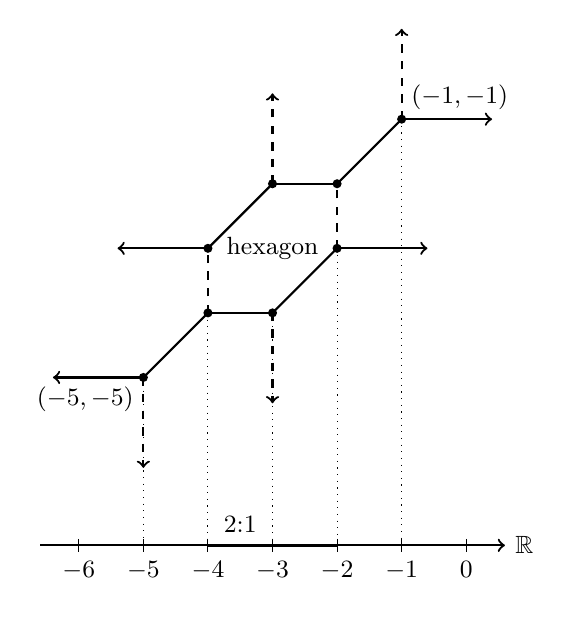
\begin{tikzpicture}[scale=0.82]
\tikzset{cont/.style={thick,dashed},edge/.style={thick}}
% bounded edges
\draw[edge] (-1,-1) -- (-2,-2);
\draw[cont] (-2,-3) -- (-2,-2);
\draw[edge] (-2,-3) -- (-3,-4);
\draw[edge] (-2,-2) -- (-3,-2);
\draw[edge] (-3,-4) -- (-4,-4);
\draw[edge] (-3,-2) -- (-4,-3);
\draw[cont] (-4,-4) -- (-4,-3);
\draw[edge] (-4,-4) -- (-5,-5);
% ends
\draw[edge,->] (-1,-1) -- (0.4,-1);
\draw[cont,->] (-1,-1) -- (-1,0.4);
\draw[edge,->] (-2,-3) -- (-0.6,-3);
\draw[cont,->] (-3,-4) -- (-3,-5.4);
\draw[cont,->] (-3,-2) -- (-3,-0.6);
\draw[edge,->] (-4,-3) -- (-5.4,-3);
\draw[cont,->] (-5,-5) -- (-5,-6.4);
\draw[edge,->] (-5,-5) -- (-6.4,-5);
% vertices
\foreach \p in {(-1,-1),(-2,-2),(-2,-3),(-3,-2),(-3,-4),(-4,-3),(-4,-4),(-5,-5)}
  \fill \p circle (2pt);
\node[above right] at (-1,-1) {\small$(-1,-1)$};
\node[below left] at (-5,-5) {\small$(-5,-5)$};
\node at (-3,-3) {\small hexagon};
% projection
\draw[thick,->] (-6.6,-7.6) -- (0.6,-7.6) node[right] {\small$\R$};
\foreach \x in {-6,-5,-4,-3,-2,-1,0} {
  \draw (\x,-7.5) -- (\x,-7.7) node[below] {\small$\x$};
}
\foreach \x/\y in {-1/-1,-2/-3,-3/-4,-4/-4,-5/-5} {
  \draw[dotted] (\x,\y) -- (\x,-7.6);
}
\draw[very thick] (-4,-7.6) -- (-2,-7.6);
\node[above] at (-3.5,-7.55) {\small$2{:}1$};
\end{tikzpicture}
\caption{The tropical curve $\Gamma$ of Example~\ref{ex:tropical} and its
projection $\pi(w)=w_1$ to the line. Dashed segments are contracted by $\pi$.
They are the two vertical sides of the hexagon and the four vertical ends.
Dotted lines show where vertices project. Every point of the line other than
$-4$ and $-2$ has exactly two preimages, so $\pi$ has degree $2$. The hexagon,
the only cycle, is folded two-to-one onto $[-4,-2]$.}\label{fig:tropical}
\end{figure}

\paragraph{What the degree of a projection says about toric codes.}
Over $\Fq$ the same projection gives a bound on zeros, by the fiber argument
behind Lemma~\ref{lem:grid}.

\begin{proposition}[Fiber bound; proved here]\label{prop:fiber}
Let $f=\sum_{u\in U}c_ux^u$ be a nonzero Laurent polynomial over $\Fq$, and let
$h=\max_{u\in U}u_2-\min_{u\in U}u_2$. If no binomial $x-c$ with $c\in\Fqs$
divides $f$, then $f$ has at most $h(q-1)$ zeros on $T(\Fq)$. More generally,
let $v\in\Z^2$ be primitive and let $v'$ be a primitive vector with $\langle
v,v'\rangle=0$. If no binomial $\chi^{v'}-c$ with $c\in\Fqs$ divides $f$, then
$f$ has at most $h_v(q-1)$ zeros, where
$h_v=\max_{u\in U}\langle v,u\rangle-\min_{u\in U}\langle v,u\rangle$. The best
choice of $v$ gives the lattice width of $\conv(U)$.
\end{proposition}

\begin{proof}
Fix $c\in\Fqs$. The Laurent polynomial $f(c,y)$ in $y$ is not zero, because
otherwise $x-c$ would divide $f$. It is $y^{\min u_2}$ times a polynomial of
degree at most $h$, so it has at most $h$ zeros in $\Fqs$. Summing over the
$q-1$ values of $c$ gives the bound. For the general statement, choose
$g\in\GL_2(\Z)$ with $gv'=(1,0)$. Then $\langle v,u\rangle$ becomes $\pm$ the
second coordinate of $gu$, and the monomial change of
coordinates of Proposition~\ref{prop:equiv}(ii) turns $\chi^{v'}-c$ into $x-c$.
This reduces the general case to the first.
\end{proof}

Lift $f$ to a polynomial over $K$ with the same support. By
Proposition~\ref{prop:projharmonic}, the degree of the projection of its
tropical curve is the vertical extent of the Newton polygon of $f$. This is at
most $h$, with equality when $f$ has nonzero terms in the top and bottom rows
of $U$.
Castryck and Cools showed that the gonality of a curve with Newton polygon
$\Delta$ is at most the lattice width of $\Delta$~\cite{CC12}.

\begin{example}\label{ex:fiberbound}
For $U=[0,2]^2$ over $\F_8$, a section with no factor $x-c$ has at most
$2\cdot7=14$ zeros on the torus, and a random search attains $14$ (script
\texttt{lattice\_width.py}). A product $(x-a)(x-b)(y-c)(y-e)$ has $24$ zeros,
which gives $d=25$ in agreement with Theorem~\ref{thrm:hansen}(c). So the
minimum-weight words come from sections with binomial factors, and every
irreducible section with Newton polygon $[0,2]^2$ gives a word of weight at
least $49-14=35$. For the principal triangle $\conv\{(0,0),(4,1),(1,4)\}$ the
lattice width is $4$, attained in the directions $(1,0)$ and $(0,1)$. Here the
fiber bound gives $4\cdot7=28$ zeros, while the true maximum is $21$
(Example~\ref{example:fan7}). A generic curve with this Newton polygon has
genus $6$, and its tropical curve has first Betti number $6$.
\end{example}

\begin{remarkxxvi}\label{rem:tropical}
The following connection has not been developed. Baker's specialization
lemma~\cite{Ba08} compares ranks of divisors on a curve and on the dual graph
of a semistable model, and it implies that gonality can only drop under
specialization to graphs. Chan characterized tropical hyperelliptic curves by
harmonic morphisms of degree two to trees~\cite{Ch13}, and
Example~\ref{ex:tropical} is a genus-one instance of that picture. A curve
with a map of degree $\gamma$ to $\PP^1$ defined over $\Fq$ has at most
$\gamma(q+1)$ rational points. So low-degree harmonic morphisms of skeleta,
when they lift to maps defined over $\Fq$, bound the number of zeros of
irreducible sections. Example~\ref{ex:fiberbound} shows that the coordinate
projection alone is not sharp for the principal code.
\end{remarkxxvi}

\begin{question}\label{q:tropical}
Can divisorial gonality, or degrees of harmonic morphisms of the skeleton
graphs computed by chip-firing, give bounds for the number of torus points on
irreducible sections that are sharper than those of~\cite{LS06}
and~\cite{SS09} for small $q$, such as $q=8$?
\end{question}

%======================================================================
\section{Summary of results and open questions}\label{sec:summary}

This section lists the status of each result and the computations behind it.
It ends with open questions. Every computation is exact over the stated
finite field. Every one is exhaustive except the searches for decoding pairs
and the random trials, which are marked as such. The scripts are in the archive accompanying this
draft.
\begingroup\raggedright
\begin{itemize}[leftmargin=*,itemsep=0pt]
\item \texttt{gf.py}: finite field arithmetic. \texttt{toric.py}: generator
matrices of toric codes.
\item \texttt{mindist.c}: exact minimum distance by an information-set search
with disjoint information sets, and weight distributions for $q=2^e$.
\item \texttt{verify\_tables.py}, \texttt{wd\_principal.py},
\texttt{minwords\_principal.py}, \texttt{minwords\_explain.py},
\texttt{automorphisms\_principal.py}: the tables and the principal example.
\item \texttt{verify\_referee.py}, \texttt{verify\_referee2.py},
\texttt{verify\_hansen.py}, \texttt{gv\_check.py} and
\texttt{resolve\_fan.py}: counterexamples, Hansen's formulas, the Gilbert--Varshamov comparison, the
fans, and the coordinate changes and moment checks of this draft.
\item \texttt{certify.py} with \texttt{certify.c}: independent verifier for
the principal code and the decoding pair (Section~\ref{sec:repro}).
\item \texttt{tropical\_example.py}, \texttt{lattice\_width.py}: the
tropical example and the fiber bound.
\item \texttt{verify\_af.py}: the Alon--F\"uredi minima, coloring counts and
cube coverings of Section~\ref{sec:nullstellensatz}.
\item For decoding, the scripts \texttt{decode\_example.py},
\texttt{decode\_pair\_check.py},
\texttt{decode\_search.py} and \texttt{decode\_\allowbreak simplex\_\allowbreak search.py}
give the worked example and the searches for pairs.
\end{itemize}
\endgroup
On $300$ random small codes, the script \texttt{test\_mindist.py} found
that \texttt{mindist.c} agrees with brute force.

\subsection{Reproducibility of the computations over \texorpdfstring{$\F_8$}{F8}}\label{sec:repro}

The computer results are exact but are not proofs. This note records what is
needed to repeat the ones for the principal code. An independent verifier
repeats them with code that shares nothing with \texttt{mindist.c},
\texttt{gf.py} or \texttt{toric.py}.
\begin{itemize}[leftmargin=*,itemsep=2pt]
\item \emph{Field and indexing.} $\F_8=\F_2[\omega]/(\omega^3+\omega+1)$, with
$\omega$ primitive. An element $c_0+c_1\omega+c_2\omega^2$ is stored as the
integer $c_0+2c_1+4c_2$. The torus point $(\omega^i,\omega^j)$ is indexed by
$(i,j)\in(\Z/7)^2$, with $i$ the outer and $j$ the inner loop. The scripts use
fixed primitive polynomials for all fields, listed in \texttt{gf.py}. In the
syndrome array of Example~\ref{ex:decode}, rows are indexed by $B_0$ and
columns by $A_0$, in the orders displayed there.
\item \emph{Commands.} In the folder \texttt{scripts/}, run
\begin{center}
\texttt{gcc -O3 -o mindist mindist.c; python3 wd\_principal.py}\\
\texttt{gcc -O3 -o certify certify.c; python3 certify.py}
\end{center}
The first line takes about $25$ seconds on one core, the second about $75$
seconds. The second pair builds the
generator matrices with its own field arithmetic. It enumerates all $8^{11}$
codewords as $\F_2$-combinations of $33$ vectors in Gray-code order, storing
each word as three $64$-bit masks.
\item \emph{Results.} Both programs give exactly the distribution of
Table~\ref{tab:wd}. The verifier also checks the three conditions of
Theorem~\ref{thm:decode} for the pair with $t=6$ in Example~\ref{ex:decode}.
It checks $A_0+B_0\subseteq P_0$ and $d(C_{A_0})=28$. It also checks that all
$\binom{49}{6}=13{,}983{,}816$ sets of six columns of the generator matrix of
$C_{B_0}$ are independent, so $d(C_{B_0}^\perp)>6$. Exactly $7$ of the
$\binom{49}{7}$ sets of seven columns are dependent, so
$d(C_{B_0}^\perp)=7$.
\item \emph{Checksums.} The SHA-256 hash of the generator matrix of the
principal code, as the nested list printed by \texttt{certify.py}, is
\texttt{a2bdf90c\ldots57de50}. The file \texttt{CHECKSUMS.txt} in the same
folder lists the SHA-256 hashes of all scripts and saved outputs.
\item \emph{Consistency checks.} As further internal checks, the table
satisfies $\sum_wA_w=8^{11}$, $\sum_wwA_w=49\cdot7\cdot8^{10}$ and
$\sum_ww(w-1)A_w=49\cdot48\cdot7^2\cdot8^9$, and $7\mid A_w$ for $w>0$
(script \texttt{verify\_referee2.py}). The first two moments hold for every
$[49,11]_8$ code with no zero coordinate. The third holds because the dual
code has minimum distance at least $3$.
\end{itemize}

\begin{center}
\small
\begin{tabular}{@{}p{0.42\textwidth}p{0.52\textwidth}@{}}
\toprule
Result & Status\\
\midrule
Lemma~\ref{lem:orth}, Props.~\ref{prop:dim}, \ref{prop:equiv},
\ref{remark:subcode}, Thm.~\ref{thm:dual} & proved here\\
Theorem~\ref{thrm:hansen}(a)--(c) & cited \cite{Ha02}; reproved here
(Prop.~\ref{prop:hansenabc})\\
Theorem~\ref{thrm:hansen}(d) & cited \cite{Ha02}; checked numerically
(Remark~\ref{rem:hansend})\\
Lemma~\ref{lem:grid}, Theorems~\ref{thrm:subcode2}, \ref{thm:segment} &
proved here\\
Estimates (i), (ii) of Section~\ref{sec:fail} & false (Examples~\ref{ex:conj1},
\ref{ex:conj2}; also \cite{Ru07})\\
Tables in Section~\ref{sec:examples} & exhaustive exact computation\\
$[49,11,28]_8$ & $k$ and $d\le28$ proved; $d\ge28$ and
Table~\ref{tab:wd} by exhaustive computation, repeated by an independent
verifier (Section~\ref{sec:repro})\\
Theorem~\ref{thm:decode}, Cor.~\ref{cor:toricECP}, Lemma~\ref{lem:separate}
& proved here\\
Example~\ref{ex:decode} & verified by computation; the conditions for
$t=6$ also by the independent verifier\\
Prop.~\ref{prop:cyclic} & proved here\\
Example~\ref{ex:minwords} & exhaustive exact computation\\
Theorems~\ref{thm:AF}, \ref{thm:BCPS} & cited \cite{AF93}, \cite{BCPS18}\\
Prop.~\ref{prop:AFgrid}; Examples~\ref{ex:cube}, \ref{ex:colorings} & proved
here; numbers checked by \texttt{verify\_af.py}\\
Prop.~\ref{prop:projharmonic}, Prop.~\ref{prop:fiber} & proved here (using the
cited facts (T2), (T3) for the first)\\
Example~\ref{ex:tropical}, Example~\ref{ex:fiberbound} & verified by
computation\\
Remarks~\ref{rem:hansend}--\ref{rem:tropical} (2026.$n$) & not fully verified, or
open\\
\bottomrule
\end{tabular}
\end{center}

\paragraph{Open questions.}
\begin{enumerate}[leftmargin=*]
\item Find error-correcting pairs, or other polynomial-time decoders, that
decode the $[49,11,28]_8$ code beyond $6$ errors, ideally up to $13$.
\item Determine the full automorphism group of the $[49,11,28]_8$ code, and
decide whether permutation decoding is practical for it.
\item Explain in general when wrap-around modulo $q-1$ creates minimum words
in directions that are not edge directions, as for the trinomials of
Example~\ref{ex:minwords}.
\item Question~\ref{q:tropical} on graph gonality and point counts.
\end{enumerate}

%======================================================================
\section{Glossary}\label{sec:glossary}

\begin{description}[leftmargin=1.5em,labelindent=0pt,style=nextline]
\item[Alon--F\"uredi theorem] A lower bound for the number of points of a grid
$A_1\times\dots\times A_r$ at which a polynomial of total degree $d$ is
nonzero, provided it is nonzero somewhere on the grid: the minimum of
$y_1\cdots y_r$ over integers $1\le y_j\le|A_j|$ with
$\sum_jy_j\ge\sum_j|A_j|-d$~\cite{AF93}. Products of linear factors in single
variables attain it. A later version also bounds the degree in each variable,
and both versions give Lemma~\ref{lem:grid} and the minimum distance of
Reed--Muller codes (Section~\ref{sec:nullstellensatz}).
\item[Cartier divisor] A torus-invariant divisor $G=\sum d_iD_i$ is Cartier if
on each maximal cone $\sigma$ it is the divisor of a single character, that is,
if there is $m_\sigma\in M$ with $\langle m_\sigma,v_i\rangle=-d_i$ for the
rays of $\sigma$. On a nonsingular toric variety every torus-invariant divisor
is Cartier. On a singular one the condition becomes a congruence, as in
Example~\ref{example:fan1}.
\item[Cayley graph] For a group $\Lambda$ and a generating set $S$, the Cayley
graph has vertex set $\Lambda$ and an edge from $s$ to $s+g$ for each $g\in S$.
The Cayley graph of $(\Z/(q-1))^r$ with $S=\{\pm e_i\}$ is the discrete torus,
the product of $r$ cycles of length $q-1$. Its translations act transitively
on the vertices, and every full-torus toric code inherits this symmetry
(Proposition~\ref{prop:cyclic}). For $q-1\le2$ the cycles degenerate, and the
graph is a single vertex or a cube.
\item[Character] A character of the torus $T$ is a homomorphism
$T\to\overline{\F}^\times$, and the characters are the monomials $\chi^u=x^u$,
$u\in M$. On the finite group $T(\Fq)$ the character $\chi^u$ depends only on
$u$ modulo $q-1$. Distinct characters of $T(\Fq)$ are linearly independent,
which is the basis of Proposition~\ref{prop:dim}.
\item[Combinatorial Nullstellensatz] Alon's theorem says that if $f$ has degree
$t_1+\dots+t_r$ and a nonzero coefficient at $x_1^{t_1}\cdots x_r^{t_r}$, then
$f$ does not vanish on all of a grid $A_1\times\dots\times A_r$ with
$|A_i|>t_i$~\cite{Al99}. It is a standard tool for list coloring and other
problems in graph theory. The related theorem of Alon and F\"uredi counts the
nonzeros of a polynomial on a grid and contains Lemma~\ref{lem:grid}(i) as a
special case.
\item[Dual code] The dual of $C\subseteq\Fq^n$ is
$C^\perp=\{v:\ v\cdot c=0\ \text{for all}\ c\in C\}$, a code of dimension
$n-\dim C$. A parity check matrix of $C$ is a generator matrix of $C^\perp$.
For full-torus toric codes the dual is again a toric code,
$C_U^\perp=C_{U^*}$ (Theorem~\ref{thm:dual}).
\item[Dual subdivision] The heights $\operatorname{val}(c_u)$ of the
coefficients of $f$ lift the lattice points of the Newton polygon to $\R^3$,
and the lower faces of the convex hull project to a subdivision of the
polygon. Its cells correspond to the vertices, edges and ends of the tropical
curve of $f$, and each edge of the curve is perpendicular to the dual edge. A
subdivision into triangles of area $1/2$ is a unimodular triangulation, as in
Example~\ref{ex:tropical}.
\item[Error-correcting pair] A pair of function spaces $(V_A,V_B)$ with
$V_AV_B\subseteq V_P$ satisfying conditions (A)--(C) of
Theorem~\ref{thm:decode}. The notion is due to Pellikaan~\cite{Pe92}, who
abstracted the error-locator algorithms for Reed--Solomon and
algebraic-geometry codes. With such a pair, decoding up to $t$ errors needs
only the solution of linear systems.
\item[Fan] A finite collection of strongly convex rational polyhedral cones in
$N_\R$, closed under taking faces, in which any two cones meet in a common
face. A fan determines a toric variety, which is complete when the cones cover
$N_\R$ and nonsingular when every cone is spanned by part of a basis of $N$.
In dimension two a complete fan is a cyclically ordered list of rays
(Section~\ref{sec:fangraph}).
\item[Generalized toric code] The code $C_U$ spanned by the evaluation vectors
of the monomials $x^u$, $u\in U$, at the points of $T(\Fq)$, for an arbitrary
finite set $U$ of exponents. When $U$ is the set of lattice points of a
polygon, it is a standard toric code. As $U$ varies over all sets of
residues, these codes are exactly the translation-invariant codes on the
discrete torus (Proposition~\ref{prop:cyclic}). The standard toric codes are
only some of them.
\item[Gonality] The gonality of an algebraic curve is the smallest degree of a
nonconstant map from the curve to the projective line. For a curve with
Newton polygon $\Delta$ it is at most the lattice width of $\Delta$~\cite{CC12}.
The divisorial gonality of a graph is the analogous invariant defined with
Baker--Norine divisors.
\item[Graph polynomial] For a graph with vertices $v_1,\dots,v_n$, the
product $f_G=\prod(x_i-x_k)$ over the edges $\{v_i,v_k\}$ with $i<k$. A choice
of colors $x_i$ from lists $L_i$ is a proper coloring exactly when $f_G$ is
nonzero there. So colorings from lists are the nonzeros of $f_G$ on a grid,
and the Combinatorial Nullstellensatz and the Alon--F\"uredi theorem apply
(Example~\ref{ex:colorings}).
\item[Harmonic morphism] A map of graphs that sends each edge to an edge or to
a vertex, such that for every vertex $x$ the number of edges at $x$ mapping
onto a given edge at the image of $x$ does not depend on that edge. It is the
graph analogue of a holomorphic map of Riemann surfaces. It has a
well-defined degree and satisfies a Riemann--Hurwitz formula~\cite{BN09}. For
metric graphs one allows integer dilation factors on edges
(Definition~\ref{def:harmonic}), and projections of tropical curves are
examples (Proposition~\ref{prop:projharmonic}).
\item[Lattice width] The width of a lattice polygon $\Delta$ in the direction
of a primitive vector $v$ is $\max_{u\in\Delta}\langle v,u\rangle-
\min_{u\in\Delta}\langle v,u\rangle$, and the lattice width is the minimum of
these widths over all primitive $v$. It is
invariant under unimodular changes of coordinates. The square $[0,2]^2$ has
lattice width $2$, and the triangle $\conv\{(0,0),(4,1),(1,4)\}$ has lattice
width $4$.
\item[Metric graph] A finite graph in which each edge is identified with a
segment of positive length, possibly together with unbounded ends. A planar
tropical curve becomes a metric graph when each edge is given its lattice
length divided by its weight; when all weights are $1$ this is just the
lattice length. The first Betti number of a metric graph plays the role of the
genus.
\item[Minimum distance] The smallest weight of a nonzero codeword of a linear
code. A code of minimum distance $d$ corrects up to $\lfloor(d-1)/2\rfloor$
errors by nearest-codeword decoding. For a toric code, $d$ is $n$ minus the
largest number of zeros on $T(\Fq)$ of a nonzero function in $V_U$.
\item[Minkowski length] The Minkowski length of a lattice polygon is the
largest number of summands of positive dimension in a Minkowski decomposition
of it. The full Minkowski length $L$ is the maximum over all lattice
subpolygons. For large $q$, Soprunov and Soprunova proved
$d\ge(q-1)^2-L(q-1)-2\sqrt q+1$ for toric surface codes~\cite{SS09}.
\item[Monomial equivalence] Two codes are monomially equivalent if one is
obtained from the other by permuting coordinates and multiplying coordinates
by nonzero scalars. Equivalent codes have the same length, dimension and
weight distribution. Lattice-equivalent exponent sets give monomially
equivalent toric codes (Proposition~\ref{prop:equiv}).
\item[Newton polygon] The Newton polygon of $f=\sum c_ux^u$ is the convex hull
of the exponents $u$ with $c_u\ne0$. It governs the geometry of the curve
$f=0$ in the torus. A generic curve with Newton polygon $\Delta$ has genus
equal to the number of interior lattice points of $\Delta$.
\item[Puncturing] Puncturing a code at a set $S$ of coordinates deletes those
coordinates from every codeword. It lowers the minimum distance by at most
$|S|$. A full-torus code of a simplex is a punctured generalized Reed--Muller
code (Theorem~\ref{thrm:subcode2}(3)).
\item[Riemann--Hurwitz formula] For a harmonic morphism $\varphi:G\to G'$ of
degree $d$ between graphs of genera $g$ and $g'$, Baker and Norine proved
$2g-2=d(2g'-2)+\sum_x\bigl(2(m_\varphi(x)-1)+v_\varphi(x)\bigr)$, where
$v_\varphi(x)$ is the number of vertical edges at $x$~\cite{BN09}. It mirrors
the classical formula for branched covers of Riemann surfaces.
Example~\ref{ex:tropical} checks it for a map of degree two from a graph of
genus one to a path.
\item[Shortening] Shortening a code at a set $S$ of coordinates keeps the
codewords that vanish on $S$ and then deletes $S$. The shortened code has
dimension at least $\dim C-|S|$ and minimum distance at least $d(C)$. The dual
of a shortened code is the punctured dual code.
\item[Standard toric code] The code obtained by evaluating the functions of
$L(G)$ at all $(q-1)^r$ points of $T(\Fq)$, for a torus-invariant divisor $G$.
Its dimension is the number of residues of $P_G\cap M$ modulo $q-1$. Only the
polytope $P_G$ matters, not the fan or the smoothness of $X$.
\item[Toric variety] A normal variety containing a torus
$T\cong(\overline{\F}^\times)^r$ as a dense open subset, such that the action
of $T$ on itself extends to the variety. Toric varieties correspond to fans,
and their geometry is encoded in the combinatorics of cones and polytopes.
Projective space, products of projective lines and Hirzebruch surfaces are
examples.
\item[Tropical curve] The tropical curve of $f=\sum c_ux^u$ over a valued field
is the set of $w\in\R^2$ where the minimum of
$\operatorname{val}(c_u)+\langle u,w\rangle$ is attained at least twice. It is a
balanced weighted planar graph with unbounded ends, dual to a subdivision of
the Newton polygon. By Kapranov's theorem it is the closure of the image of
the curve $f=0$ under coordinatewise valuation~\cite{MS15}.
\item[Weight] The Hamming weight of a vector is the number of its nonzero
coordinates. The Hamming distance between two vectors is the weight of their
difference. The weight distribution of a code lists, for each $w$, the number
$A_w$ of codewords of weight $w$ (Table~\ref{tab:wd}).
\end{description}

%======================================================================
\section*{Acknowledgments}
\addcontentsline{toc}{section}{Acknowledgments}

I thank S{\o}ren Hansen, Johan Hansen and Amin Shokrollahi for answering many
questions, and for helpful correspondence regarding their research.

This corrected and expanded version was prepared with AI assistance. OpenAI
ChatGPT (GPT-6) acted as referee. It wrote a report on the 2003 manuscript,
and a second report on the revised drafts that led to the corrections of
Draft~4. Anthropic Claude (Claude Opus~5.5) acted as reviser. It checked each
point of both reports independently and wrote the revised text. It found the grid-lemma
proofs, the duality and cyclic-code statements, the decoding theorem in its
present form and its worked example, and the graph-theoretic material of
Section~\ref{sec:graphs}. It also wrote and ran the verification scripts. AI
review is not an independent certification of the results. Further details on
the AI usage, including which sources could not be consulted, can be found in
the revision log.

%======================================================================
\begingroup\raggedright
\begin{thebibliography}{GAP00}

\bibitem[ABBR15]{ABBR15}
O.~Amini, M.~Baker, E.~Brugall\'e and J.~Rabinoff, Lifting harmonic morphisms
I: metrized complexes and Berkovich skeleta, \emph{Res. Math. Sci.}
\textbf{2} (2015), Art.~7.

\bibitem[Al99]{Al99}
N.~Alon, Combinatorial Nullstellensatz, \emph{Combin. Probab. Comput.}
\textbf{8} (1999), 7--29.

\bibitem[AF93]{AF93}
N.~Alon and Z.~F\"uredi, Covering the cube by affine hyperplanes,
\emph{European J. Combin.} \textbf{14} (1993), 79--83.

\bibitem[Ba08]{Ba08}
M.~Baker, Specialization of linear systems from curves to graphs, \emph{Algebra
Number Theory} \textbf{2} (2008), 613--653.

\bibitem[AT92]{AT92}
N.~Alon and M.~Tarsi, Colorings and orientations of graphs,
\emph{Combinatorica} \textbf{12} (1992), 125--134.

\bibitem[BCPS18]{BCPS18}
A.~Bishnoi, P.~L.~Clark, A.~Potukuchi and J.~R.~Schmitt, On zeros of a
polynomial in a finite grid, \emph{Combin. Probab. Comput.} \textbf{27}
(2018), 310--333.

\bibitem[BN09]{BN09}
M.~Baker and S.~Norine, Harmonic morphisms and hyperelliptic graphs,
\emph{Int. Math. Res. Not. IMRN} (2009), no.~15, 2914--2955.

\bibitem[BCP97]{BCP97}
W.~Bosma, J.~Cannon and C.~Playoust, The Magma algebra system I: The user
language, \emph{J. Symbolic Comput.} \textbf{24} (1997), 235--265.

\bibitem[Br98]{Br98}
A.~E.~Brouwer, Bounds on the size of linear codes, in \emph{Handbook of
Coding Theory}, V.~Pless and W.~C.~Huffman, eds., North-Holland, 1998. Online
tables formerly at \texttt{http://www.win.tue.nl/\~{}aeb/voorlincod.html}.

\bibitem[BK13]{BK13}
G.~Brown and A.~M.~Kasprzyk, Small polygons and toric codes, \emph{J.
Symbolic Comput.} \textbf{51} (2013), doi:10.1016/j.jsc.2012.07.001.

\bibitem[BK13b]{BK13b}
G.~Brown and A.~M.~Kasprzyk, Seven new champion linear codes, \emph{LMS J.
Comput. Math.} (2013), arXiv:1212.5197.

\bibitem[CC12]{CC12}
W.~Castryck and F.~Cools, Newton polygons and curve gonalities, \emph{J.
Algebraic Combin.} \textbf{35} (2012), 345--366.

\bibitem[Ch13]{Ch13}
M.~Chan, Tropical hyperelliptic curves, \emph{J. Algebraic Combin.}
\textbf{37} (2013), 331--359.

\bibitem[DGM70]{DGM70}
P.~Delsarte, J.-M.~Goethals and F.~J.~MacWilliams, On generalized Reed--Muller
codes and their relatives, \emph{Inform. and Control} \textbf{16} (1970),
403--442.

\bibitem[Ew96]{Ew96}
G.~Ewald, \emph{Combinatorial Convexity and Algebraic Geometry}, Springer,
1996.

\bibitem[FL98]{FL98}
J.~Fitzgerald and R.~F.~Lax, Decoding affine variety codes using Gr\"obner
bases, \emph{Des. Codes Cryptogr.} \textbf{13} (1998), 147--158.

\bibitem[Fu93]{Fu93}
W.~Fulton, \emph{Introduction to Toric Varieties}, Princeton University
Press, 1993.

\bibitem[GAP00]{GAP00}
The GAP Group, \emph{GAP -- Groups, Algorithms, and Programming, Version
4.3}, 2000, \texttt{http://www.gap-system.org}.

\bibitem[GUA02]{GUA02}
GUAVA, a GAP package for computing with error-correcting codes, Version 1.6,
2002.

\bibitem[Gr26]{Gr26}
M.~Grassl, Bounds on the minimum distance of linear codes and quantum codes,
\texttt{http://www.codetables.de}, consulted November 22, 2026.

\bibitem[Ha00]{Ha00}
J.~P.~Hansen, Toric surfaces and error-correcting codes, in \emph{Coding
Theory, Cryptography and Related Areas} (Guanajuato, 1998), Springer, 2000,
132--142.

\bibitem[Ha02]{Ha02}
J.~P.~Hansen, Toric varieties, Hirzebruch surfaces and error-correcting codes,
\emph{Appl. Algebra Engrg. Comm. Comput.} \textbf{13} (2002), 289--300.

\bibitem[Ha04]{Ha04}
J.~P.~Hansen, Toric surfaces and codes, techniques and examples, Preprint
Series No.~1, Department of Mathematics, University of Aarhus, 2004.

\bibitem[Ha13]{Ha13}
J.~P.~Hansen, Quantum codes from toric surfaces, \emph{IEEE Trans. Inform.
Theory} \textbf{59} (2013), 1188--1192.

\bibitem[Ha17]{Ha17}
J.~P.~Hansen, Toric codes, multiplicative structure and decoding, preprint,
2017, arXiv:1702.06569.

\bibitem[SH96]{SH96}
S.~H.~Hansen, Algebraic geometry over finite fields -- with a view towards
applications, Master's thesis, University of Aarhus, 1996.

\bibitem[SH99]{SH99}
S.~H.~Hansen, The geometry of Deligne--Lusztig varieties: higher-dimensional
AG codes, PhD thesis, University of Aarhus, 1999.

\bibitem[SH01]{SH01}
S.~H.~Hansen, Error-correcting codes from higher-dimensional varieties,
\emph{Finite Fields Appl.} \textbf{7} (2001), 530--552.

\bibitem[Jo02]{Jo02}
D.~Joyner, \textbf{toric}: MAGMA and GAP code for toric codes
(\texttt{toric.mag}, \texttt{toric.g}), circa 2002.

\bibitem[Jo04]{Jo04}
D.~Joyner, Toric codes over finite fields, \emph{Appl. Algebra Engrg. Comm.
Comput.} \textbf{15} (2004), 63--79.

\bibitem[JV02]{JV02}
D.~Joyner and H.~Verrill, Notes on toric varieties, preprint, circa 2002.

\bibitem[Li03a]{Li03a}
J.~Little, A key equation and the computation of error values for codes from
order domains, preprint, 2003, arXiv:math/0303299.

\bibitem[Li03b]{Li03b}
J.~Little, The ubiquity of order domains for the construction of error
control codes, preprint, 2003, arXiv:math/0304292.

\bibitem[Li11]{Li11}
J.~Little, Remarks on generalized toric codes, preprint, 2011,
arXiv:1107.4530.

\bibitem[Li17]{Li17}
J.~B.~Little, Toric codes and finite geometries, \emph{Finite Fields Appl.}
\textbf{45} (2017), arXiv:1504.07494.

\bibitem[LS06]{LS06}
J.~Little and H.~Schenck, Toric surface codes and Minkowski sums, \emph{SIAM
J. Discrete Math.} \textbf{20} (2006), 999--1014.

\bibitem[LS07]{LS07}
J.~Little and R.~Schwarz, On toric codes and multivariate Vandermonde
matrices, \emph{Appl. Algebra Engrg. Comm. Comput.} \textbf{18} (2007),
349--367.

\bibitem[Mi05]{Mi05}
G.~Mikhalkin, Enumerative tropical algebraic geometry in $\R^2$, \emph{J.
Amer. Math. Soc.} \textbf{18} (2005), 313--377.

\bibitem[MS15]{MS15}
D.~Maclagan and B.~Sturmfels, \emph{Introduction to Tropical Geometry},
Graduate Studies in Mathematics~161, American Mathematical Society, 2015.

\bibitem[MS77]{MS77}
F.~J.~MacWilliams and N.~J.~A.~Sloane, \emph{The Theory of Error-Correcting
Codes}, North-Holland, 1977.

\bibitem[Pe92]{Pe92}
R.~Pellikaan, On decoding by error location and dependent sets of error
positions, \emph{Discrete Math.} \textbf{106/107} (1992), 369--381.

\bibitem[PH98]{PH98}
V.~Pless and W.~C.~Huffman, eds., \emph{Handbook of Coding Theory},
North-Holland, 1998.

\bibitem[Ru07]{Ru07}
D.~Ruano, On the parameters of $r$-dimensional toric codes, \emph{Finite
Fields Appl.} \textbf{13} (2007), 962--976.

\bibitem[Ru09]{Ru09}
D.~Ruano, On the structure of generalized toric codes, \emph{J. Symbolic
Comput.} \textbf{44} (2009), 499--506.

\bibitem[SV90]{SV90}
A.~N.~Skorobogatov and S.~G.~Vl\u{a}du\c{t}, On the decoding of
algebraic-geometric codes, \emph{IEEE Trans. Inform. Theory} \textbf{36}
(1990), 1051--1060.

\bibitem[SS09]{SS09}
I.~Soprunov and J.~Soprunova, Toric surface codes and Minkowski length of
polygons, \emph{SIAM J. Discrete Math.} \textbf{23} (2009), 384--400.

\bibitem[St93]{St93}
H.~Stichtenoth, \emph{Algebraic Function Fields and Codes}, Springer, 1993.

\end{thebibliography}
\endgroup

\end{document}
